%%%%%%%%%%%%%%%%%%%%%%%%% 
% Dokumentinformationen % 
%%%%%%%%%%%%%%%%%%%%%%%%% 
\newcommand{\titleinfo}{Stochastic Modeling}
\newcommand{\authorinfo}{S. Eicher, L. Schmid, R. Koller, Ch. Schlittler, S. Carriero} % Do not remove any names! Initial authors stay first.
\newcommand{\versioninfo}{FS2014}

%%%%%%%%%%%%%%%%%%%%%%%%%%%%%%%%%%%%%%%%%%%%%
% Standard projektübergreifender Header für
% - Makros 
% - Farben
% - Mathematische Operatoren  
%
% DORT NUR ERGÄNZEN, NICHTS LÖSCHEN
%%%%%%%%%%%%%%%%%%%%%%%%%%%%%%%%%%%%%%%%%%%%%  

% Genereller Header
\documentclass[10pt,twoside,a4paper,fleqn]{article}
\usepackage[utf8x]{inputenc}
\usepackage[left=1cm,right=1cm,top=1cm,bottom=1cm,includeheadfoot]{geometry}
\usepackage[ngerman]{babel,varioref}
\usepackage[T1]{fontenc}


% Pakete
\usepackage{amssymb} 
\usepackage{amsmath}
\usepackage{fancybox}
\usepackage{graphicx}
\usepackage{color}
\usepackage{lastpage}
\usepackage{wrapfig}
\usepackage{fancyhdr}
\usepackage{hyperref}
\usepackage{verbatim}
\usepackage{floatflt}
\usepackage{arydshln}
\usepackage{ucs}
\usepackage{pdflscape} % landscape
\usepackage{multirow} % zellen in tabellen verbinden
\usepackage{multicol} 
%\usepackage{pgf,tikz} %Zeichnen

% \usepackage{slashbox} % getrennte zelle in tabelle
% \usepackage{array} % anordnung in tabellen

%%%%%%%%%%%%%%%%%%%%
% Generelle Makros %
%%%%%%%%%%%%%%%%%%%%


\newcommand{\skript}[1]{$_{\textcolor{red}{\mbox{\small{Script p. #1}}}}$}
\newcommand{\sachs}[1]{$_{\textcolor{blue}{\mbox{\small{Sachs S. #1}}}}$}
\newcommand{\formelbuch}[1]{$_{\textcolor{red}{\mbox{\small{S#1}}}}$}
\newcommand{\verweis}[2]{ {\small (siehe auch \ref{#1}, #2 (S. \pageref{#1}))}}
\newcommand{\subsubadd}[1]{\textcolor{black}{\mbox{#1}}}
\newenvironment{liste}[0]{\begin{list}{$\bullet$}{\setlength{\itemsep}{0cm}\setlength{\parsep}{0cm} \setlength{\topsep}{0cm}}}{\end{list}}
    
\newcommand{\logd}[0]{\log_{10}}
\newcommand{\subsubsubsection}[1]{\textbf{#1}}

\newenvironment{aufzaehlung}[0]{\begin{enumerate}{\setlength{\itemsep}{0cm}\setlength{\parsep}{0cm}\setlength{\topsep}{0cm}}} {\end{enumerate}}

\newcommand{\abbHeight}[3]{
	\begin{center}
		\includegraphics[height=#2]{./bilder/#1} \\
		#3
    \end{center}
}


\newcommand{\skriptsection}[2]{\section{#1 \formelbuch{#2}}}
\newcommand{\skriptsubsection}[2]{\subsection{#1 \formelbuch{#2}}}
\newcommand{\skriptsubsubsection}[2]{\subsubsection{#1 \formelbuch{#2}}}

%%%%%%%%%%
% Farben %
%%%%%%%%%%
\definecolor{black}{rgb}{0,0,0}
\definecolor{red}{rgb}{1,0,0}
\definecolor{white}{rgb}{1,1,1}
\definecolor{grey}{rgb}{0.8,0.8,0.8}

%%%%%%%%%%%%%%%%%%%%%%%%%%%%
% Mathematische Operatoren %
%%%%%%%%%%%%%%%%%%%%%%%%%%%%
\DeclareMathOperator{\sinc}{sinc}
\DeclareMathOperator{\sgn}{sgn}



% Fouriertransformationen
\unitlength1cm
\newcommand{\FT}
{
\begin{picture}(1,0.5)
\put(0.2,0.1){\circle{0.14}}\put(0.27,0.1){\line(1,0){0.5}}\put(0.77,0.1){\circle*{0.14}}
\end{picture}
}


\newcommand{\IFT}
{
\begin{picture}(1,0.5)
\put(0.2,0.1){\circle*{0.14}}\put(0.27,0.1){\line(1,0){0.45}}\put(0.77,0.1){\circle{0.14}}
\end{picture}
}
\newcommand{\jw}{j\omega}

\newcommand{\DFT}
{
%\overset{DFT}{
	\begin{picture}(1,0.2)
	\put(0.2,0.1){\circle{0.14}}{\put(0.27,0.1){\line(1,0){0.5}}}\put(0.77,0.1){\circle*{0.14}}
	\end{picture}
%}
}

\newcommand{\IDFT}
{
%\overset{IDFT}{
    \begin{picture}(1,0.2)
	\put(0.2,0.1){\circle*{0.14}}\put(0.27,0.1){\line(1,0){0.45}}\put(0.77,0.1){\circle{0.14}}
	\end{picture}
%}
}


\newcommand{\twopartdef}[4]
{
	\left\{
		\begin{array}{ll}
			#1 & \mbox{if } #2 \\
			#3 & \mbox{if } #4
		\end{array}
	\right.
}

\newcommand{\mtwopartdef}[3]
{
	\left\{
		\begin{array}{ll}
			#1 & \mbox{if } #2 \\
			#3 & \mbox{otherwise }
		\end{array}
	\right.
}

\newcommand{\threepartdef}[6]
{
	\left\{
		\begin{array}{lll}
			#1 & \mbox{if } #2 \\
			#3 & \mbox{if } #4 \\
			#5 & \mbox{if } #6
		\end{array}
	\right.
}

\newcommand{\bm}{\boldsymbol}
\newcommand{\todo}[2][red]{\textcolor{#1}{TODO: #2}}
\newcommand{\numbercircled}[1]{\textcircled{\raisebox{-1pt}{#1}}}



%%%%%%%%%%%%%%%%%%%%%%%%%%%%
% Allgemeine Einstellungen %
%%%%%%%%%%%%%%%%%%%%%%%%%%%%
%pdf info
\hypersetup{pdfauthor={\authorinfo},pdftitle={\titleinfo},colorlinks=false}
\author{\authorinfo}
\title{\titleinfo}

%Kopf- und Fusszeile
\pagestyle{fancy}
\fancyhf{}
%Linien oben und unten
\renewcommand{\headrulewidth}{0.5pt} 
\renewcommand{\footrulewidth}{0.5pt}


\fancyhead[L]{\titleinfo{ }- Summary}
%Kopfzeile rechts bzw. aussen
\fancyhead[R]{\today{ }- Page \thepage/\pageref{LastPage}}
\fancyfoot[C]{\copyright{ }\authorinfo}

% Einrücken verhindern versuchen
\setlength{\parindent}{0pt}


% Einheiten
%#########################################################################################
\usepackage[Gray,squaren]{SIunits} %\gray befehl heisst nun \Gray

%Spannung
\DeclareMathOperator{\V}{\volt}
\DeclareMathOperator{\mV}{\milli \volt}
\DeclareMathOperator{\uV}{\micro \volt}

%Strom
\DeclareMathOperator{\A}{\ampere}
\DeclareMathOperator{\mA}{\milli \ampere}
\DeclareMathOperator{\uA}{\micro \ampere}
\DeclareMathOperator{\nA}{\micro \ampere}

%Zeit
\DeclareMathOperator{\s}{\second}
\DeclareMathOperator{\ms}{\milli \second}
\DeclareMathOperator{\us}{\micro \second}
\DeclareMathOperator{\ns}{\nano \second}

%Kapazität
\DeclareMathOperator{\mF}{\milli \farad}
\DeclareMathOperator{\uF}{\micro \farad}
\DeclareMathOperator{\nF}{\nano \farad}
\DeclareMathOperator{\pF}{\pico \farad}
\DeclareMathOperator{\fF}{\femto \farad}

%Induktivität
\DeclareMathOperator{\mH}{\milli \henry}
\DeclareMathOperator{\uH}{\milli \henry}
\DeclareMathOperator{\nH}{\nano \henry}

%Widerstand
\DeclareMathOperator{\MO}{\mega \ohm}
\DeclareMathOperator{\kO}{\kilo \ohm}
\DeclareMathOperator{\mO}{\milli \ohm}

%Strecke
\DeclareMathOperator{\km}{\kilo \meter}
\DeclareMathOperator{\cm}{\centi \meter}
\DeclareMathOperator{\mm}{\milli \meter}

%Frequenz
\DeclareMathOperator{\GHz}{\giga \hertz}
\DeclareMathOperator{\MHz}{\mega \hertz}
\DeclareMathOperator{\Hz}{\hertz}
\DeclareMathOperator{\kHz}{\kilo \hertz}
\DeclareMathOperator{\mHz}{\milli \hertz}

%Leistung
\DeclareMathOperator{\kW}{\kilo \watt}
\DeclareMathOperator{\mW}{\milli \watt}
\DeclareMathOperator{\uW}{\micro \watt}

%Kreisfrequenz
\DeclareMathOperator{\rpers}{\radianpersecond}

%DeziBel
\DeclareMathOperator{\dB}{\deci \bel}

\DeclareMathOperator{\e}{\mathrm e}


   

% Möglichst keine Ergänzungen hier, sondern in header.tex
\begin{document} 

%%%%%%%%%%%%%%%%%%%%%%%%%%%%%%%%%%%%%%%%%%%%%%%%%%%%%%%%%%%%%%%%%%%%%%%%%%%%%%%%%%%%%%%%%%%%%%%
%%%%%%%%%%%%%%%%%%%%%%%%%%%%%%%%%%%%%%%%%%%%%%%%%%%%%%%%%%%%%%%%%%%%%%%%%%%%%%%%%%%%%%%%%%%%%%%


\section{Events and Probability}
$P(A)=\frac{k}{n}=\frac{\text{number of good outcomes}}{\text{total number of possible outcomes}}=\frac{|A|}{|\Omega|}$\\

\vspace{5mm}
 
	\begin{minipage}{8cm}
	\subsection{Probability \skript{16}}
		\begin{tabular}{ll}
			Codomain (Wertebereich):
			& ${0}\le{P(A)}\le{1}$\\ \\
			Certain (Sicheres) event:
			& $P(\Omega)=1$\\ \\
			Impossible event:
			& $P(\emptyset)=0$\\
			Subset (Untermenge) $A\subseteq B$: & $P(A)\leq P(B)$
		\end{tabular}
	\end{minipage}
		\begin{minipage}{11.2cm}
		\subsubsection{Calculation rules}
			\begin{tabular}{ll}
				Complementary event: &$P(\bar{A})=P({\Omega}\setminus{A})=1-P(A)$\\ \\
				Difference: &$P({A}\setminus{B})=P(A)-P({A}\cap{B})$\\ \\
				OR: &$P({A}\cup{B})=P(A)+P(B)-P({A}\cap{B})$\\
				AND (independent): & $P(A\cap B)=P(A)P(B)$
				
			\end{tabular}
		\end{minipage}
		\newline
		
\vspace{2mm}
\hrule

\vspace{3mm}


	\subsection{Independent events \skript{22}}
		\begin{minipage}{12cm}
			$A$ and $B$ are independent if:\\
			
			$P(A \mid B)=P(A)$ and $P(B \mid A)=P(B)$ is true.\\
			
			Then: \hspace*{8mm} $P(A\cap B)=P(A)P(B)$\\
		\end{minipage}
		\begin{minipage}{4cm}
			$ \cap \equiv AND $ \\
			$ \cup \equiv OR $\newline
		\end {minipage}\\
    	Die Tatsache, dass A eingetreten ist, hat keinen Einfluss auf die 
		Wahrscheinlichkeit von B.\\ 

		\vspace{2mm}
		\hrule
		\vspace{3mm}
		
	\subsection{Conditional probability of A given B / Bedingte Wahrscheinlichkeit \skript{18}}
		Die Wahrscheinlichkeit für das Eintreten des Ereignisses $A$ unter der
		Bedingung, dass das Ereignis $B$ bereits eingetreten ist.
		\begin{center}
		$P(A\mid B)= \dfrac{P(A\cap B)}{P(B)}=\underbrace{\frac{P(A)\cdot
		P(B)}{P(B)}=P(A)}_{\text{nur wenn unabhängig}}$ 
		\end{center}

	\vspace{2mm}
	\hrule
	\vspace{3mm}

\subsection{Bayes rule (Wahrscheinlichkeitsumkehr) \skript{18}}
		\begin{tabular}{ll}
		  $P(B\mid A)=P(A\mid B) \cdot\dfrac{P(B)}{P(A)} = \dfrac{P(A|B) P(B)}{\sum\limits_{i=1}^n P(A|B_i) P(B_i)}$\vspace{1mm}
		\end{tabular}
		
	\vspace{2mm}
	\hrule
	\vspace{3mm}

\subsection{Law of total probability \skript{19}}
  \begin{minipage}{10cm}
	  \begin{tabular}{ll}
			$P(E)=\sum\limits_{i=1}^n P(E\mid A_i)\cdot P(A_i)$ \\
			Example: \\
			$P(E)=P(E\mid X)\cdot P(X)+P(E\mid !X)\cdot P(!X)$
	  \end{tabular}
  \end{minipage} 
  \begin{minipage}{10cm}
  	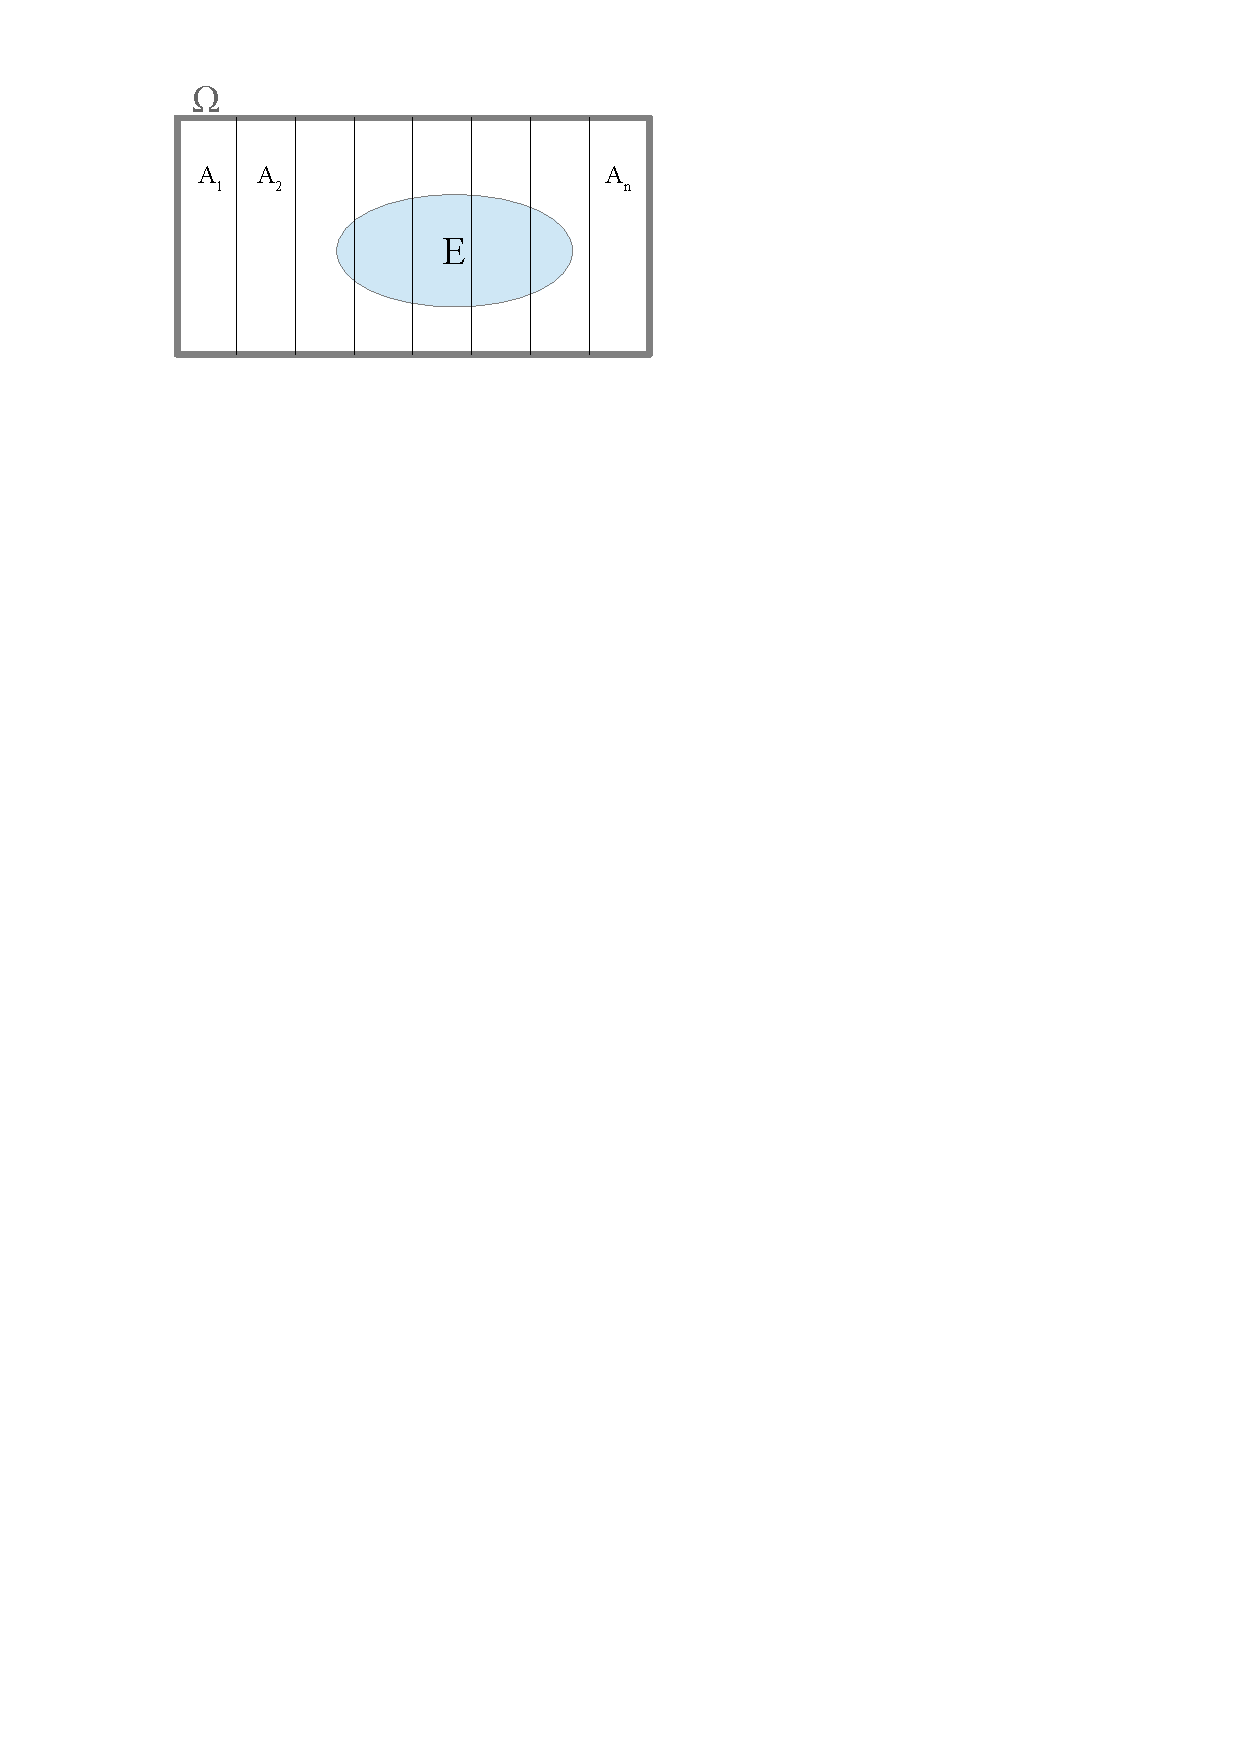
\includegraphics[width=5cm]{./Content/EreignisseWahrscheinlichkeit/total_probability.pdf}
  \end{minipage}
	
	\vspace{2mm}
	\hrule
	\vspace{3mm}
				
\subsection{Laplace event}
		In einem endlichen Wahrscheinlichkeitsraum $\Omega$ haben alle
		Elementarereignisse die gleiche Wahrscheinlichkeit.
		\begin{center}
		$P(A)=\dfrac{\left| A\right|}{\left|\Omega\right|}$
		\end{center}
		
	\vspace{2mm}
	\hrule
	\vspace{3mm}

\vfill
\newpage
	
	


\section{Random variables \skript{25,26}}

\begin{tabular}{p{5.5cm}p{8.5cm}p{4cm}}
$X: \Omega \rightarrow \mathbb{R}$&	$X=\{x_1, \ldots, x_n, \ldots\}$&\\
&&\\
	Discrete random variable (RV): &$P(X=x_i)=P(\{\omega|X(\omega)=x_i\})$& $i=\{1,2,\ldots,n,\ldots\}$\\
	Continuous random variable (RV): &$P(X\in [a,b])=P(\{\omega|X(\omega)=X\in a,b]\})=\int\limits_a^b{f(x)}dx$& $i=[a,b]$ \\
									&																			&$f(x)$: density function.
\end{tabular}

\begin{tabular}{p{5.5cm}p{4cm}p{4cm}}
Normalization:&$\sum\limits_{i=1}^\infty{P(X=x_i)}=1$& $\int\limits_{-\infty}^\infty{f(x)dx}=1$\\
\end{tabular}

\vspace{2mm}
\hrule
\vspace{3mm}

\subsection{Cumulative Distribution Function (Verteilungsfunktion): F(x) \skript{26,27}}

	\begin{tabular}{p{3cm}p{6cm}}
	
	Discrete: &$F(x)=P(X\leq x)=\sum\limits_{x_i:x_i\leq x}{P(X=x_i)}$\\
	Continuous: &$F(x)=P(X\leq x)=\int\limits_{-\infty}^x{f(x)dx}$\\
	\end{tabular}
	
	\renewcommand{\arraystretch}{1.5}
	\begin{tabular}[]{|l|l|}
	      	\hline
	      	\textbf{Discrete} & \textbf{Continuous}\\
	      	\hline
	      	\hline
	      	$P(X\leq x)=F_X(x)=\sum\limits_{k=-\infty}^x p_k$ &
	      	$P(X\leq x)=F_X(x)=\int\limits_{-\infty}^x
	      	f_X(\tilde{x})d\tilde{x}$\\
				$P(X>x)=1-P(X\leq x)$ & $P(X>x)=1-P(X\leq x)$\\        	
	      	$P(a \le X \leq b)=F_X(b)-F_X(a)=\sum\limits_{k=a}^b p_k$ &
				$P(a \le X \leq b)=F_X(b)-F_X(a)=\int \limits_a^b
				f_X(\tilde{x})d\tilde{x}$\\
	      	\hline
	\end{tabular}
	\renewcommand{\arraystretch}{1}

\subsubsection{Properties}
	$$\boxed{\mathbb{D}(F) = \mathbb{R}} \qquad \boxed{\mathbb{W}(F)
	\in[0,1]} \qquad \boxed{F(-\infty)=0} \qquad  \boxed{F(\infty)=1}
	\qquad \boxed{F(x) \text{ increases monotonically}}$$

\hrule

\vspace{5mm}
	\begin{minipage}{13cm}
	\subsubsection{Probability density function}
		\begin{tabular}{p{3.3cm}p{8.5cm}}
    	$f_X(x)=F'(x)$ & probability density function \\
    	
    	\multirow{2}{11cm}{\textbf{At jump discontinuity of $F_X(x)$: }}\\
    	\multirow{2}{11cm}{$\varphi(x) = $ delta impulse with value of the jump heigh}
    	
    	\end{tabular}
	\end{minipage}
	\begin{minipage}{5cm}
		\subsubsection{Expectation}
			\begin{tabular}{ll}
            $E(X)=\int\limits_{-\infty}^{\infty}{x f_X(x)dx}$\\
        	$E(X^2)=\int\limits_{-\infty}^{\infty}{x^2 f_X(x)dx}$\\
			$E(X^N)=\int\limits_{-\infty}^{\infty}{x^N f_X(x)dx}$\\
        	\end{tabular}
	\end{minipage}
\hrule
\vspace{2mm}

	\subsubsection{Calculation rules for $f_X$ und $F_X$}
		\begin{minipage}{11cm}
			\begin{tabular}{lll}
        	Given: & X, Y Random variables, 
        	&$f_X$, $f_Y$ known\\
        	\end{tabular}\\
 
        	\begin{tabular}{p{6cm}p{6cm}}
        	Probability function: & Density function:\\
        	$F_{X+a}(x)=F_X(x-a)$  &$f_{X+a}(x)=f_X(x-a)$\\
        	$F_{\lambda X}(x)=F_X(\frac{x}{\lambda})$ &$f_{\lambda
        	X}(x)=f_X(\frac{x}{\lambda})\frac{1}{\lambda}$\\
        	$F_{X+Y}(x)=F_X\ast f_Y(y)=F_Y\ast f_X(x)$ &
        	$f_{X+Y}(x)=f_X\ast f_Y(x)$\\
        	$F_{\sqrt{X}}(x)=F_X(x^2)$ &
        	$f_{\sqrt{X}}(x)=2x f_X(x^2)$\\
        	$F_{X^2}(x)=F_X(\sqrt{x})$ &
        	$f_{X^2}(x)=\frac{1}{2}x^{-\frac{1}{2}}f_X(\sqrt{x})$
        	\end{tabular}
		\end{minipage}
		\begin{minipage}{7cm}
        	\subsubsection{Example algorithm}
        	\begin{tabular}{ll}
        	1. Use definition of $F$: $F_{\lambda X}(x)=P(\underbrace
        	{\lambda X\leq x}_{*})$\\[0.5cm]
        	2. Transform * definition: $P(X \leq
        	\frac{x}{\lambda})=F_X(\frac{x}{\lambda})$\\[0.5cm]
        	3. For density: $\frac{d}{dx}$\\[0.5cm]
        	$f_{\lambda X}(x)=\frac{d}{dx}F_{\lambda
        	X}(x)=\frac{d}{dx}F_X(\frac{x}{\lambda})=
        	f_X(\frac{x}{\lambda})\frac{1}{\lambda}$
        	\end{tabular}
			\vspace{10mm}
        \end{minipage}
        
		\subsubsection{Maximum of an interval}
		$X_1,\ldots X_i$ sind auf dem Intervall $[0,l]$ mit $F_X(x)$ verteilt: $M=\max \{ X_1,\ldots,X_i\} $; $F_M(x)=F_X(x)^n$
\vspace{2mm}
\hrule
\vspace{3mm}

\subsection{Expectation: E(x) \skript{27}}
\begin{minipage}{12cm}
  \begin{tabular}{p{2cm}p{4cm}p{5cm} }
  			&  Expectation (1. moment)						&	$n$-th moment	\\
  Discrete:	 &$E(X)=\sum\limits_{i=1}^\infty{x_i P(X=x_i)}$	&	$E(X^n)=\sum\limits_{i=1}^\infty{x_i^n P(X=x_i)}$\\
  Continuous:  &$E(X)=\int\limits_{-\infty}^\infty{x f(x)dx}$	&	$E(X^n)=\int\limits_{-\infty}^\infty{x_i^n f(x)dx}$\\
  \end{tabular}
\end{minipage}
\begin{minipage}{7cm}
  $E(X+Y)=E(X)+E(Y)$\\
  $E(\lambda X + \mu)=\lambda \cdot E(X) + \mu \qquad\lambda, \mu \in \mathbb{R}$\\
  $E(XY) = E(X)\cdot E(Y)$ (if independent)\\
\end{minipage}

\vspace{2mm}
\hrule
\vspace{3mm}

\subsection{Variance: V(X)=Var(X) \skript{27,28}}
  \begin{tabular}{p{2cm}p{8cm}l}
  	$Var(X)$	&	$=E(X^2)-E^2(X)=E\left([X-E(X)]^2\right)$						& \\
  	Discrete: 	&	$V(X)=Var(X)=\sum\limits_{i=1}^\infty{(x_i-E(X))^2 P(X=x_i)}$	& \\
  	Continuous: &	$V(X)=Var(X)=\int\limits_{-\infty}^\infty{(x_i-E(X))^2 f(x)dx}$	& \\
  \end{tabular}

\begin{minipage}{12cm}
    $Var(X+Y)= \begin{cases}
                  Var(X)+Var(Y)
                  & \text{(X,Y independent)}\\                     
                  Var(X) + Var(Y) + 2 \cdot Cov(X,Y) 
                  & \text{(X,Y dependent)}\\
               \end{cases} $ \\
    $Var(X Y)= Var(Y)Var(X)+Var(Y)E(X)^2+Var(X)E(Y)^2$
\end{minipage}
\begin{minipage}{7cm}
    $Var(\lambda X)=\lambda^2 Var(X) \qquad $ $\lambda \in
    \mathbb{R}$\\ 
    $Var(X_1+X_2+\ldots+X_n) \neq Var(n X)$ \\
\end{minipage}
\vspace{2mm}
\hrule
\vspace{3mm}

\subsection{Moment Generating Function $\phi(t)$ \skript{28}}
Used to calculate first or second order moments (mean, variance). If a MGF can be
derived, then the distribution is unique.

\begin{tabular}{p{5cm}p{12cm}}
Discrete: &$\phi(t)=E(\e^{tX})=\sum\limits_{i=1}^\infty{\e^{t x_i} P(X=x_i)}$\\
Continuous: &$\phi(t)=E(\e^{tX})=\int\limits_{-\infty}^\infty{\e^{t x} f(x)dx}$\\
Summation of processes: & $\phi_{X \pm Y}(t) = E(\e^{t(X \pm Y)}) = E(\e^{tX}) E(\e^{t(\pm Y)})=\phi_{X}(t)\cdot\phi_Y(\pm t)$ \\
Example: &$E(X)=\left.\phi'(t)\right|_{t=0} \qquad E(X^2)=\left.\phi''(t)\right|_{t=0} \qquad E(X^n)=\left.\phi^{(n)}(t)\right|_{t=0}$
\end{tabular}

	\vspace{2mm}
	\hrule
	\vspace{3mm}
	

\subsection{Covariance (Abhängigkeit) $Cov(X,Y)$ \skript{36-38}}
\begin{minipage}{12.5cm}
  $Cov(X,Y)=E(XY)-E(X)E(Y)=E([X-E(X)][Y-E(Y)])$ 

  \begin{tabular}{p{2cm}p{9.5cm}}
  Discrete: &$Cov(X,Y)=\sum\limits_{x_i,y_j}{(x_i-E(X))(y_j-E(Y))P({X=x_i,Y=y_i})}$\\
  
  Continuous: &$Cov(X,Y)=\int\limits_{-\infty}^\infty{\int\limits_{-\infty}^\infty{(x-E(X))(y-E(Y))f_{X,Y}(x,y)dy}dx}$\\
  \end{tabular}\\
  
  \textbf{Covariance matrix $P_X$:}\\
  $P_X=\begin{bmatrix}
          Cov(X_1,X_1) & \hdots & Cov(X_1,X_m) \\                                   
          \vdots & \ddots & \vdots \\                             
          Cov(X_m,X_1) & \hdots & Cov(X_m,X_m)
      \end{bmatrix}=E[(\mathbf{X}-E(\mathbf{X}))(\mathbf{X}-E(\mathbf{X}))^T]$
\end{minipage}
\begin{minipage}{6.5cm}
  $Cov(X,Y) > 0$: correlated\\
  $Cov(X,Y) = 0$: uncorrelated\\
  $Cov(X,Y) < 0$: correlated inversely\\
  $Cov(X,X) = Var(X)$: identical\\
  
  $Cov(X,Y) = Cov(Y,X)$ \\
$Cov(aX,Y) = a Cov(X,Y)$ \\
$Cov(\sum_i X_i, \sum_j Y_j) = \sum_i \sum_j Cov(X_i, Y_i)$\\
\end{minipage}

\vspace{2mm}
\hrule
\vspace{3mm}
	
	
\subsection{Correlation Coefficient $\rho$ \skript{38}}
\begin{minipage}{8cm}
  $-1\leq\boxed{\rho=\displaystyle\frac{Cov(X,Y)}{\sqrt{Var(X)}\sqrt{Var(Y)}}}=cos(\varphi)\leq 1$\\
\end{minipage}
\begin{minipage}{10cm}
  if $X$, $Y$ independent: $\rho=0$ \qquad if $X=Y$: $\rho = 1$

  \textbf{WSS} (wide sense stationary): $\rho_X(t_1, t_2)=\frac{C_X(t_2-t_1)}{C_X(0)}$\\
\end{minipage}

\vspace{2mm}
\hrule
\vspace{3mm}

\subsubsection{Jointly distributed random variables \skript{36}}
$F(a,b)=P(X \leq a, Y \leq b) = P(X \leq a \cap Y \leq b) \quad -\infty < a,b < \infty $\\
$p(x,y)=P(X=x, Y=y)$\\
$P(\{X \in [a,b], Y \in [c,d]\})= \int\limits_a^b \int\limits_c^d f(x,y)dy dx $

\vspace{2mm}
\hrule

\subsection{Autocorrelation}
	$\boxed{R_X(t_1,t_2)=E\left[(X_{t_1} X_{t_2}\right]}$\\
	\vspace{0.2cm}
	Estimation of the autocorrelation of a WSS process $X_k$:\\
\begin{minipage}{9cm}
	\textbf{discrete}	\\
	$\boxed{\hat{R}_X(n):=\frac{1}{2N+1} \displaystyle\sum_{k=-N}^{N}X_{k+n}X_k} $ is equal to\\
	$\boxed{\frac{1}{2N+1} \displaystyle\sum_{k=-N}^{N} E(X_{k+n}X_k) = \displaystyle\sum_{k=-N}^{N} R_X(n) = R_X(\tau)} $
\end{minipage}
\hspace{0.5cm}
\begin{minipage}{9cm}
	\textbf{continuous}	\\
	$\boxed{ \hat{R}_X(n):= \frac{1}{2T} \displaystyle\int_{-T}^T X_{t+\tau}X_t dt }$ is equal to\\
	$\boxed{ \frac{1}{2T} \displaystyle\int_{-T}^T E(X_{t+\tau}X_t)dt = \frac{1}{2T} \displaystyle\int_{-T}^T R_X(\tau) dt = R_X(\tau) }$
\end{minipage}

\subsubsection{Autocovariance}
$\boxed{C_X(t_1,t_2)=R_X(t_1,t_2)-E\left[X_{t_1} \right]E\left[X_{t_2}\right]}$

\vspace{2mm}
\hrule
\vspace{3mm}

\subsection{Discrete Random Variables \skript{28-32}}
\subsubsection{Bernoulli RV \skript{28,29}}
\begin{minipage}{10cm}
	\begin{liste}
		\item Throw a coin
		\item $P(X=1)=p$\\$P(X=0)=1-p$
		\item $p\in[0,1]$
	\end{liste}
\end{minipage}
\hfill
\begin{minipage}{8cm}
	\begin{liste}
		\item $E(X)=p$
		\item $Var(X)=p(1-p)$
		\item $\phi(t)=\e^{0\cdot p}(1-p)+\e^{1\cdot p}(p)=p\e^t+1-p$
	\end{liste}
\end{minipage}
\hfill

	\vspace{2mm}
	\hrule
	\vspace{3mm}

\subsubsection{Binomial RV $X\sim Binom(n,p)$ \skript{29,30}}
	\begin{liste}
			\item Summation of $n$ Bernoulli RV / number of $k$ (exactly) success that occur in $n$ trials
	\end{liste}
\begin{minipage}{12cm}
	\begin{liste}
		\item $\boxed{p(\{X=k\}) = \binom n k p^k(1-p)^{n-k}\qquad k=\{0,1,2,\ldots,n\}}$
		\vspace{0.2cm}
		\item $p\in[0,1]$
		\vspace{0.2cm}
		\item $\boxed{P\big(X\geq\alpha\big)=\sum\limits_{k=\alpha}^{n}{\binom n k p^k(1-p)^{n-k}}}=1-\sum\limits_{k=0}^{\alpha-1}{\binom n k p^k(1-p)^{n-k}}$
	\end{liste}
\end{minipage}
\hfill
\begin{minipage}{7cm}
	\begin{liste}
		\item $E(X)=np$
		\item $Var(X)=np(1-p)$
		\item $\phi(t)=n(p\e^t+1-p)^n$
	\end{liste}
\end{minipage}
\hfill\\


$n$: number of experiments \hspace{10mm}
$k$: number of success \hspace{10mm}
$p$: probability\\

\begin{minipage}{8cm}
	\scalebox{1}{
	\renewcommand{\arraystretch}{1}
	\begin{tabular}{rccccccccc}
		$n=0$:&    &    &    &    &  1\\\noalign{\smallskip\smallskip}
		$n=1$:&    &    &    &  1 &    &  1\\\noalign{\smallskip\smallskip}
		$n=2$:&    &    &  1 &    &  2 &    &  1\\\noalign{\smallskip\smallskip}
		$n=3$:&    &  1 &    &  3 &    &  3 &    &  1\\\noalign{\smallskip\smallskip}
		$n=4$:&  1 &    &  4 &    &  6 &    &  4 &    &  1\\\noalign{\smallskip\smallskip}
	\end{tabular}}
\end{minipage}
\begin{minipage}{6cm}	
	$\binom n k =\frac{n!}{k!(n-k)!}\qquad\text{TR: }nCr(n,k)$\\[0.5cm]
	$\binom n n = \binom n 0=1$\\[0.5cm]
	$\binom n k =0 \qquad k>n$\\[0.5cm]
\end{minipage}
\hfill

\textbf{Approximation of a binomial RV $X_B\sim Binom(n,p)$ with a Poisson RV  $X_P\sim Pois(\lambda=np)$}\\

$P(\{X=i\})\approx\e^{-\lambda}\frac{\lambda^i}{i!}\qquad with\qquad \lambda=np \qquad i=\{1,2,\ldots,n\}$

\vspace{2mm}
\hrule
\vspace{3mm}

\subsubsection{Poisson RV $X\sim Pois(\lambda)$ for $\lambda>0$ \skript{30,31}}

\begin{minipage}{10cm}
	\begin{liste}
		\item $\boxed{p(\{X=i\}) = \frac{\lambda^i}{i!}\e^{-\lambda}\qquad i=\{0,1,2,\ldots\}}$
		\vspace{0.2cm}
		\item $\lambda > 0$
	\end{liste}
\end{minipage}
\hfill
\begin{minipage}{8cm}
	\begin{liste}
		\item $E(X)=\lambda$
		\item $Var(X)=\lambda$
		\item $\phi(t)=\e^{\lambda(\e^t-1)}$
		\item $\max_i(p) = \{\lambda-a, \lambda\}$
	\end{liste}
\end{minipage}\\

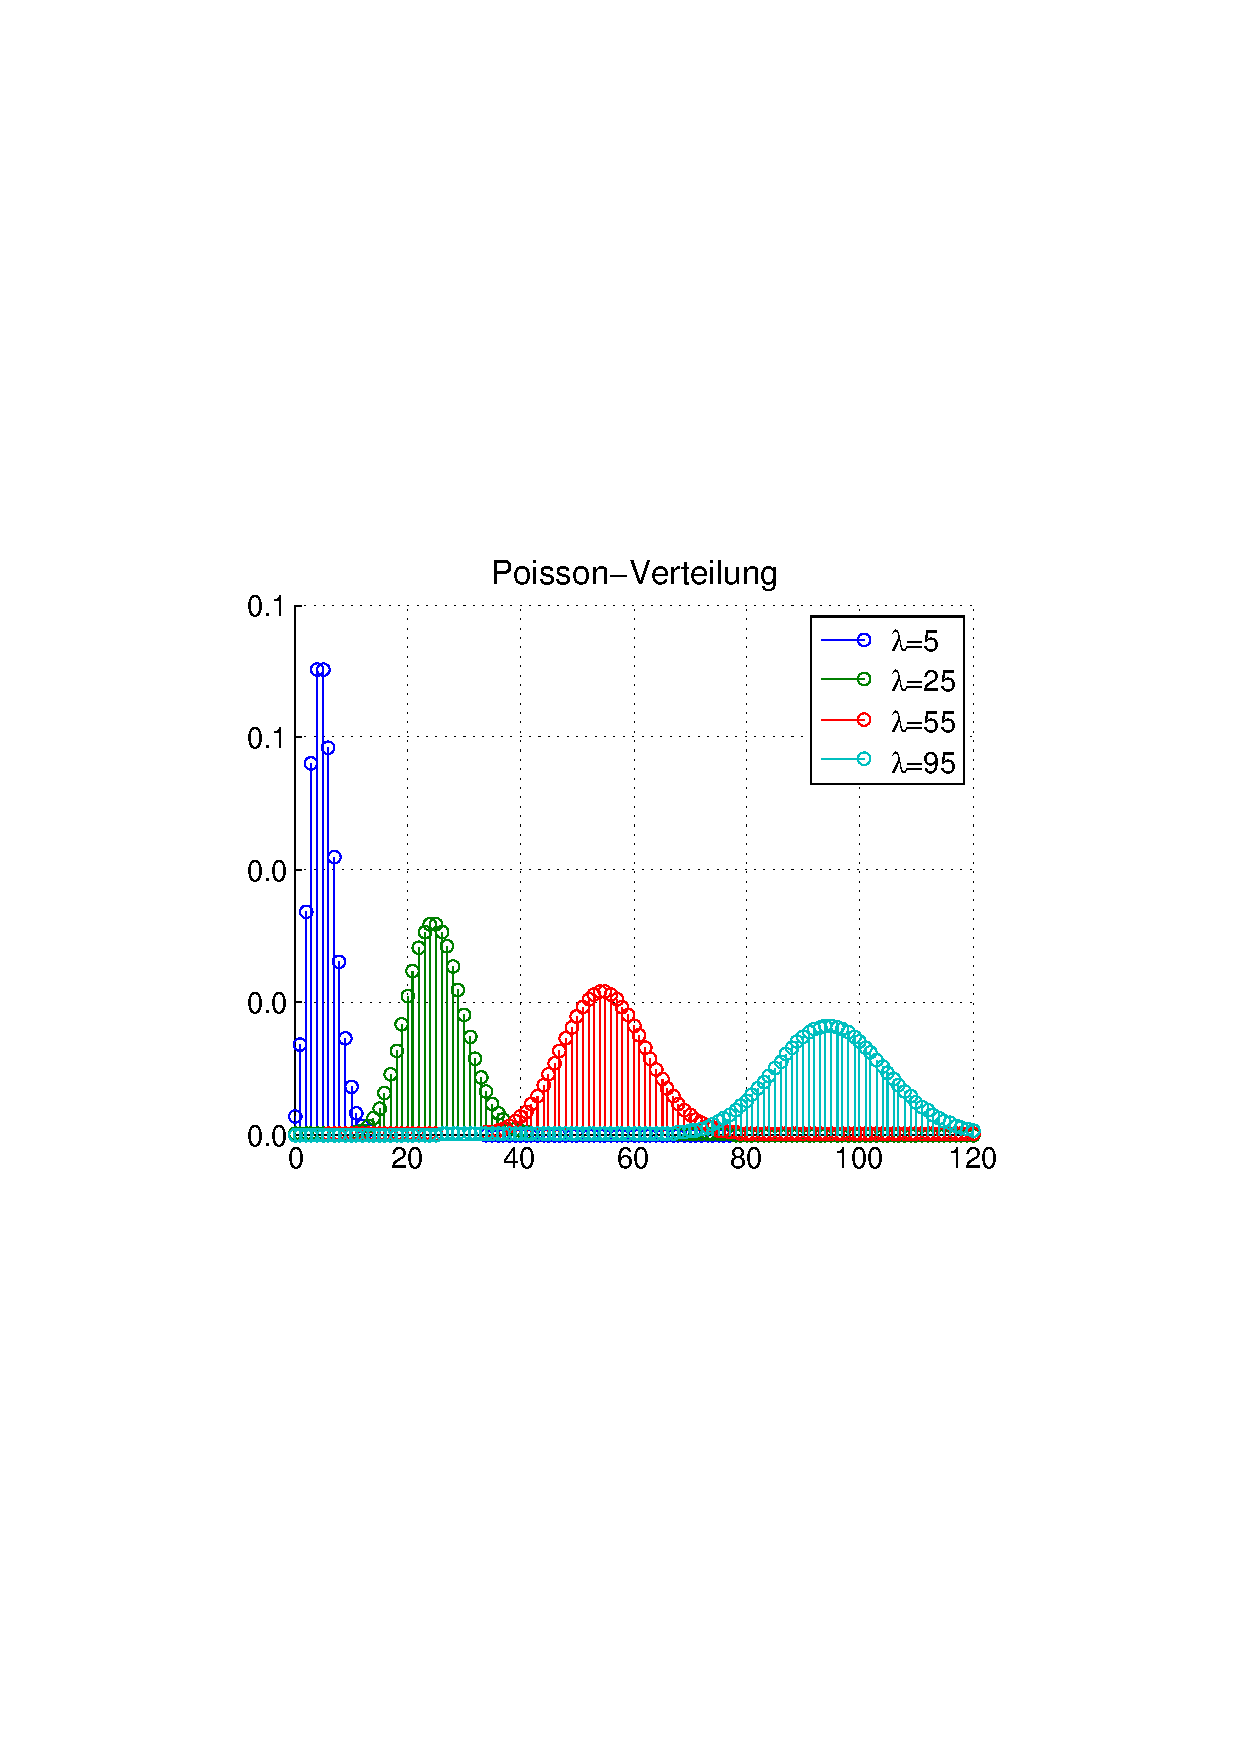
\includegraphics[width=10cm,trim=4.0cm 9.5cm 4.0cm 9.25cm ,clip]{Content/RandomVariable/Poisson}

\vspace{2mm}
\hrule
\vspace{3mm}

\subsubsection{Geometric RV $X\sim Geom(p)$ \skript{31,32}}

\begin{minipage}{10cm}
	\begin{liste}
		\item Number of independent trials required until first success
		\vspace{0.2cm}
		\item $\boxed{p(\{X=i\}) = (1-p)^{i-1}p\qquad i=\{1,2,\ldots\}}$
	\end{liste}
\end{minipage}
\hfill
\begin{minipage}{8cm}
	\begin{liste}
		\item $E(X)=\frac 1p$
		\item $Var(X)=\frac {1-p}{p^2}$
		\item $\phi(t)=\frac{p\e^t}{1-(1-p)\e^t}$
	\end{liste}
\end{minipage}
\hfill

\vspace{2mm}
\hrule
\vspace{3mm}

\subsection{Continuous Random Variables \skript{32}}
\subsubsection{Uniform RV $X\sim U(\alpha,\beta)$ \skript{32}}
\begin{minipage}{10cm}
$f_X(x) = \twopartdef { \frac{1}{\beta-\alpha} } {\alpha \leq x \leq\beta} {0} {\text{otherwise}}$
\end{minipage}
\begin{minipage}{10cm}
	\begin{liste}
		\item $E(X)=\frac {\alpha+\beta}{2}$
		\item $Var(X)=\frac {(\alpha-\beta)^2}{12}$
		\item $\phi(t)=\frac{\e^{t\beta}-\e^{t\alpha}}{t(\beta-\alpha)}$
	\end{liste}
\end{minipage}
\hfill
\vspace{2mm}
\hrule
\vspace{3mm}

\subsubsection{Exponential RV $X\sim Exp(\lambda)$ \skript{33}}
\begin{minipage}{10cm}

\begin{equation}
f_X(x) = \twopartdef { \lambda\e^{-\lambda x} } {x\geq 0} {0} {x<0}\\
F_X(x) = \twopartdef { 1-\e^{-\lambda x} } {x\geq 0} {0} {x<0}\nonumber
\end{equation}

\end{minipage}
\begin{minipage}{9cm}
	\begin{liste}
		\item $E(X)=\frac {1}{\lambda}$
		\item $Var(X)=\frac {1}{\lambda^2}$
		\item $\phi(t)=\frac{\lambda}{\lambda-t}$
		\item $\max(f_X)$ when $f_X(0)=\lambda$
		\item $P[X>s+t | X>t]= \displaystyle\frac{ \e^{-\lambda (s+t)} }{ \e^{-\lambda t} }=\e^{-\lambda s} = P[X>s]$
	\end{liste}
\end{minipage}
\hfill

\vspace{2mm}
\hrule
\vspace{3mm}

\subsubsection{Normal RV $X\sim N(\mu,\sigma^2)$ \skript{33-35}}
\begin{minipage}{10cm}
$f_X(x) = \displaystyle\frac{1}{\sqrt{2\pi}\sigma}\cdot\e^{\displaystyle\frac{-(x-\mu)^2}{2\sigma^2}}\qquad -\infty <x<\infty$
\end{minipage}
\begin{minipage}{10cm}
	\begin{liste}
		\item $E(X)=\mu$
		\item $Var(X)=\sigma^2$
		\item $\phi(t)=\e^{\frac{\sigma^2t^2}{2}+\mu t}$
	\end{liste}
\end{minipage}
\hfill

\textbf{Example:}\\
If $X\sim N(\mu,\sigma^2)$ and $Y=\alpha X+ \beta$, \qquad
then: $Y\sim N(\alpha\mu+\beta,\alpha^2\sigma^2)$\\



\subsubsection{Standard normal distribution $\Phi(x)$:}

\textbf{Normalisation:} $Y=\frac{X-\mu}{\sigma}\sim N(0,1)$ \qquad for \qquad $X\sim N(\mu,\sigma^2)$ \qquad $\Rightarrow$ \qquad
$\underbrace{\Phi(x)=\displaystyle\frac 1 {\sqrt{2\pi}}\int\limits_{-\infty}^x{\displaystyle\e^{\displaystyle\frac{-y^2}{2}}dy} }_{\text{cumulative distribution function}}$\\

\vspace{0.5cm}

\textbf{Example:} $X\sim N\big(\mu,\sigma^2\big)\quad \Rightarrow \quad P\big(\alpha<X<\beta\big)\quad\overset{Norm.}{=}\quad P\big(\frac{\alpha-\mu}{\sigma}<\frac{X-\mu}{\sigma}<\frac{\beta-\mu}{\sigma}\big)=\underbrace{\Phi\left(\frac{\beta-\mu}{\sigma}\right)-\Phi\left(\frac{\alpha-\mu}{\sigma}\right)}\limits_{\text{Std.-Normal-Distr. table}}$\\
\textbf{Bei negativen Werten:} $\boxed{\Phi(\alpha)=1-\Phi(-\alpha)}$


\vspace{2mm}
\hrule

\subsubsection{Bivariate Normal RV }

$f_{X1,X2}(x1,x2)=\displaystyle\frac{1}{2\pi\sigma_1\sigma_2\sqrt{1-\rho^2}}\cdot\e^{\displaystyle-\frac{1}{2(1-\rho^2)}\left[\left(\frac{x_1-\mu_1}{\sigma_1}\right)^2-2\rho\frac{x_1-\mu_1}{\sigma_1}\frac{x_2-\mu_2}{\sigma_2}+\left(\frac{x_2-\mu_2}{\sigma_2}\right)^2\right]}$\\

$f_{X_1|X_2}(x_1|x_2)=\displaystyle\frac{1}{\sqrt{2\pi}\cdot \sigma_1}\frac{1}{\sqrt{1-\rho^2}}\cdot\e^{\displaystyle-\frac{\left(x_1-\mu_1-\rho\frac{\sigma_1}{\sigma_2}(x_2-\mu_2)\right)^2}{2(1-\rho^2)\sigma_1^2}}$\\

$E(X_1|X_2=x_2)=\mu_1+\rho\frac{\sigma_1}{\sigma_2}(x_2-\mu_2)$ (see example 18, \formelbuch{52})\\
$Var(X_1|X_2=x_2)=\sigma_1^2(1-\rho^2)$

\vspace{2mm}
\hrule

\subsubsection{Multivariate Normal RV $\mathbf{X} \sim N(\mathbf{\mu},\mathbf{C})$}
$f_X(x)=\displaystyle\frac{1}{(2\pi)^{n/2}\sqrt{det(C)}}\cdot\e^{\displaystyle-\frac{1}{2}(x-\mu)^T\cdot C^{-1}\cdot(x-\mu)}$\\
$E(X_i)=\mu_i$\\
$Var(X_i)=\sum\limits_{j=i}^n{a_{ij}^2=C_{ii}}$\\
$\phi_X(t_1,\ldots,t_m)=E(\e^{t_1X_1+\ldots+t_mX_m})$

\vspace{2mm}
\hrule


\section{Limit Theorems \skript{43-46}}
\begin{liste}
\item The law of large numbers:
	$\Rightarrow$ Es is prinzipiell möglich, den Erwartungswert einer Zufallsvariablen durch (unendlich) oftes Wiederholen zu bestimmen.\\
	$\lim\limits_{n \rightarrow \infty}{\frac{X_1+X_2+\ldots+X_n}{n}}=\mu$
\item Central limit theorem\\
	$\Rightarrow$ Die Summe einer grossen Zahl von unabhängigen Zufallsvariablen befolgt asymptotisch eine stabile Verteilung $\to$ Normalverteilung.\\
	$\{X_1,X-2,\ldots\}$ is a sequence of independent and identically distributed RV's with $E(X_i)=\mu$ and $Var(X_i)=\sigma^2$. Then the distribution converges to the standard normal as $n\rightarrow\infty$.\\

$\lim\limits_{n \rightarrow \infty}{P\left(\frac{X_1+X_2+\ldots+X_n-n\mu}{\sigma \sqrt{n}}\leq a\right)}=\frac{1}{\sqrt{(2\pi)}}\int\limits_{-\infty}^{a}{\e^{-x^2/2}dx}$
\end{liste}

\newpage

\section{Conditional Probabilities \skript{47-62}}
$\boxed{P_{X|Y}=P(X=x|Y=y)=\frac{P(X=x,Y=y)}{P(Y=y)}}$\\

\begin{tabular}{lll}

  & \textbf{Conditional Cumulative Distribution Fct} & \textbf{Conditional Expectation}\\[0.3cm]
  
Definition & $\boxed{F_{X|Y}(x,y)=P(X \leq x|Y=y)}$ & $E(X|Y=y)$\\[0.3cm]
Continuous & $F_{X|Y}(x,y)=\int\limits_{-\infty}^{x}\frac{f(\tilde{x},y)}{f_Y(y)}d\tilde{x}$	& $E(X|Y=y) = \int\limits_{-\infty}^{\infty}xf_{X|Y}(x|y)dx = \int\limits_{-\infty}^{\infty}x\frac{f(x,y)}{f_Y(y)}dx$\\[0.5cm]
Discrete   & $F_{X|Y}(x,y)=\sum\limits_{x} \frac{P(X=x, Y=y)}{P(Y=y)}$ &	$E(X|Y=y) = \sum\limits_{x} x P(X=x|Y=y) = \sum\limits_{x} x \frac{P(X=x, Y=y)}{P(Y=y)}$\\
\end{tabular}\\

\subsection{A static estimation problem I \skript{56,57}}

One Measurement: $\boxed{Y=X+N}$	
\quad $\boxed{\hat{X}:=f(y)=E(X|Y=y) = y \frac{\sigma_X^2}{\sigma_X^2+\sigma_N^2}}$ 
with error variance $\boxed{\sigma^2=\frac{\sigma_{X}^2 \sigma_{N}^2}{\sigma_{X}^2 + \sigma_{N}^2}}$\\


Theorem: The minimum mean-square error estimator $\hat{X}$ ist the expected value of $X$ knowing the observation $Y=y$.

\subsection{A static estimation problem II \skript{58-60}}

\begin{minipage}{0.6\textwidth}
These are essential ideas behind Kalman filter. Two independent measurements ($z_1, z_2$) at different time.
A model is required: $Z = X + N$ with $Z$ as observation, $X$ the real value and $N$ noise.
	\begin{liste}
	\item Initial condition: Error variance $\sigma_x^2 = \infty$
	\item $t=t_1$:\\
	$\hat{X}(t_1)=\lim\limits_{\sigma_{X}^2 \rightarrow \infty}{E(X(t_1)|Z_1=z_1)}=\lim\limits_{\sigma_{X}^2 \rightarrow \infty}{z_1\frac{\sigma_X^2}{\sigma_X^2+\sigma_{z_1}^2}}=z_1$\\
	$\sigma_x^2(t_1)=\lim\limits_{\sigma_{X}^2 \rightarrow \infty}{\frac{\sigma_X^2 \sigma_{z_1}^2}{\sigma_X^2 + \sigma_{z_1}^2}}=\sigma_{z_1}^2$
	\item $t=t_2$:\\
	
	$\hat{X}(t_2)=\hat{X}(t_1)+K\left(z_2-\hat{X}(t_1)\right)$\\
	$K=\frac{\sigma_{z_1}^2}{\sigma_{z_1}^2 + \sigma_{z_2}^2}$
	with an associated error variance $\sigma^2=\frac{\sigma_{z_1}^2 \sigma_{z_2}^2}{\sigma_{z_1}^2 + \sigma_{z_2}^2}$
	\item Rewritten:\\
	$\hat{z}=\left(\frac{\sigma_{z_2}^2}{\sigma_{z_1}^2 + \sigma_{z_2}^2}\right)z_1 + \left(\frac{\sigma_{z_1}^2}{\sigma_{z_1}^2 + \sigma_{z_2}^2}\right) z_2$\\
	$\frac{1}{\sigma^2}=\frac{1}{\sigma_{z_1}^2} + \frac{1}{\sigma_{z_2}^2}$
	
	\end{liste}
\end{minipage}
\begin{minipage}{0.4\textwidth}
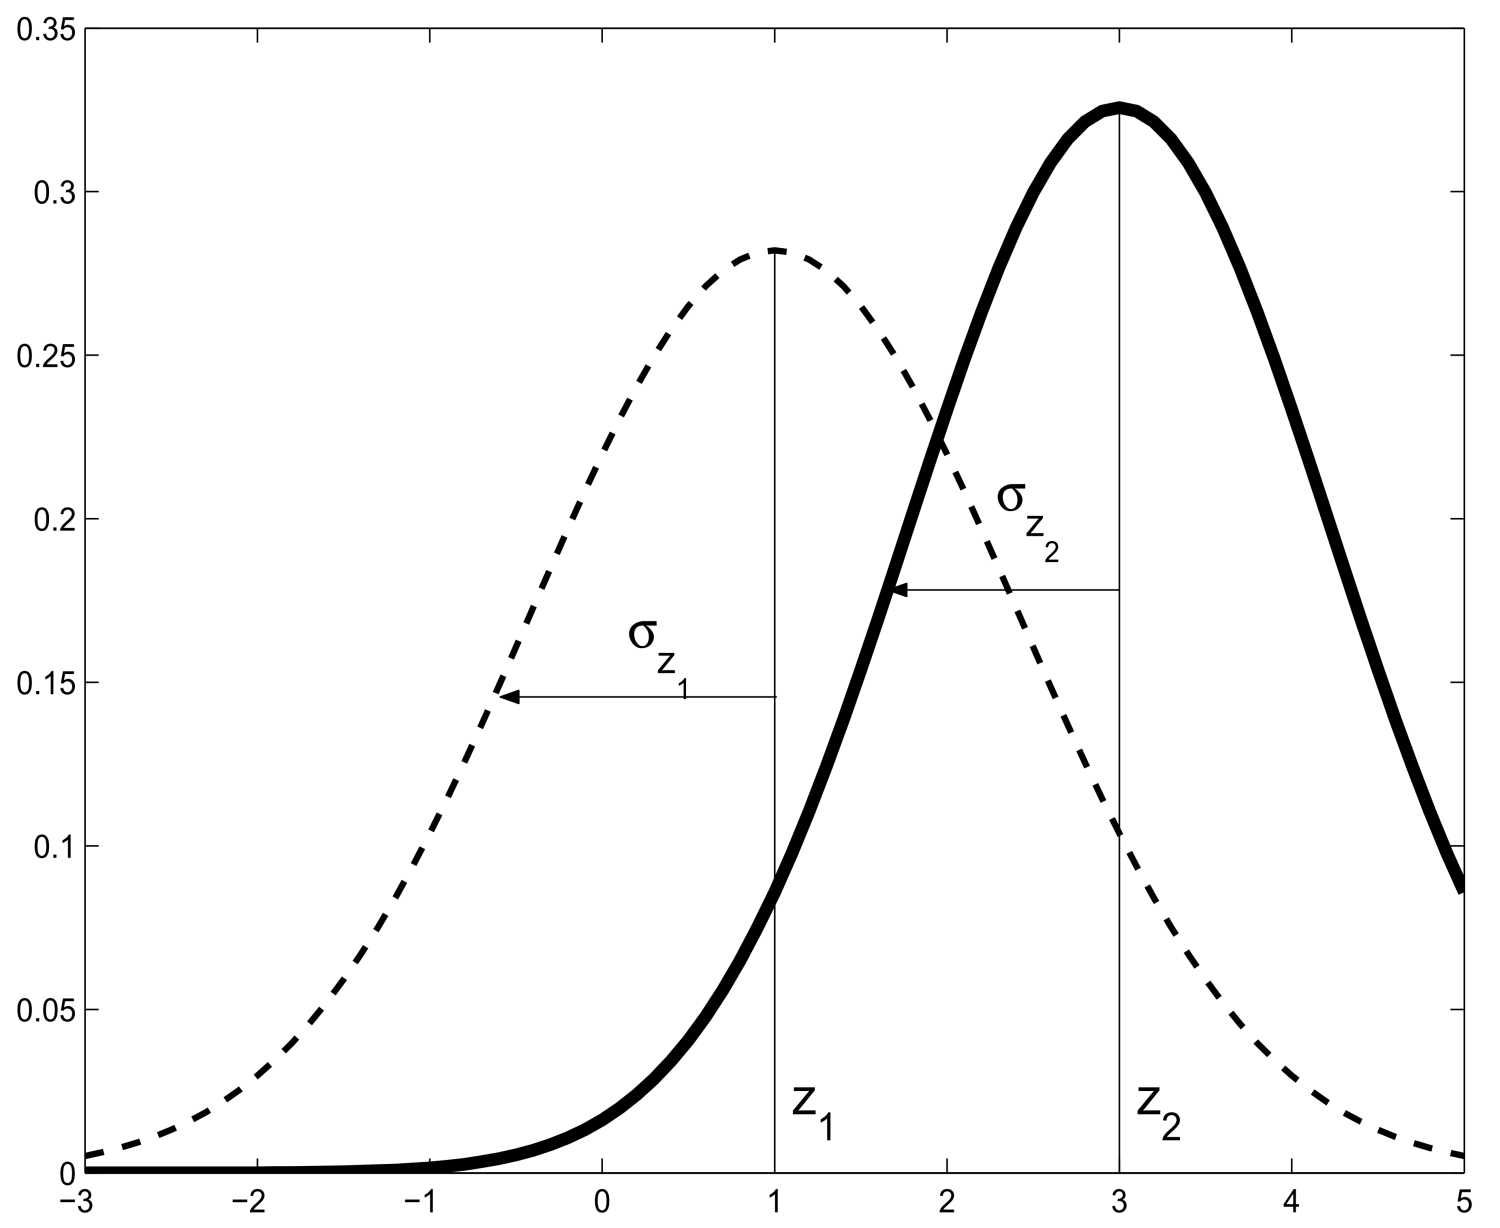
\includegraphics[width=\linewidth]{./Content/LimitTheorems/TwoMeas}
\end{minipage}

\vspace{2mm}
\hrule



\section{Stochastic Processes \skript{63-102}}

\begin{tabular}{|l|l|l|}
	\hline
					&	$\mathbb{T}$ \textit{discrete}	& $\mathbb{T}$ \textit{continuous} \\
	\hline
	$S$ \textit{discrete} 	&	 random walk			& Poisson process \\
	\hline
	$S$ \textit{continuous}	&	time series				& Brownian motion \\	
	\hline
\end{tabular}
$S$: state space, $\mathbb{T}$: time \\

\begin{tabular}{ p{4.5cm} p{8cm} l}
% 	\textbf{Mean}: 						&	$E(X_t)$		& \\
%	\textbf{Autocorrelation}:			&	$R_X(t_1,t_2)=E\left[(X_{t_1} X_{t_2}\right]$	& \\
%	\textbf{Autocovariance}: 			&	$C_X(t_1,t_2)=R_X(t_1,t_2)-E\left[X_{t_1} \right]E\left[X_{t_2}\right]$	& \\
%	\textbf{Correlation coefficient}: 	&	$\rho_X(t_1,t_2)=\frac{C_X(t_1,t_2)}{\sqrt{C_X(t_1,t_1) C_X(t_2,t_2)}}$	& 	WSS: $\rho_X(t_1, t_2)=\frac{C_X(t_2-t_1)}{C_X(0)}$\\
%										&	$|\rho| \leq 1$, 1 = perfect correlation \\
	\textbf{Average power}: 			&	$R_X(t,t)=E\left[X_t^2\right]$	& \\
	\textbf{strict sense stationary}: 	&	A stochastic process $X$ is strict sense stationary, if the finite dimensional distribution function is invariant under time shift	 \\
	\textbf{wide sense stationary (WSS)}:& 	A stochastic process $X$ ist wide sense stationary, if the mean $E(X_t)=m$ is a constant and if the autocorellation function $R_X(t_1,t_2)$ only depends on the difference $t=t_2-t_1$. Dann gilt $R_X(t)=R_X(t_1,t_1+t)$. 	& \\
	\textbf{white noise}: 				&	A wide sense stationary process $X_t$ is called white noise if $E(X_t)=0$ and $R_X(t)=C_X(t)=\frac{D}{2}\delta(t)$	& \\
\end{tabular}

\subsection{(power) spectral density}	
$R_X(t)\FT S_X(k)$ \\
\begin{tabular}{ll}
	continuous:		&	$S_X(k)=\int\limits_{-\infty}^{\infty}{\e^{-j k t}R_x(t)dt}$	\\
	discrete: 		&	$S_X(k)=\sum\limits_{n=-\infty}^{\infty}{\e^{-j 2\pi k n}R_x(n)}$	 \\
	because real:	&	$S_X(k)=\int\limits_{-\infty}^{\infty}{cos(kt)R_x(t)dt}$; \qquad $R_X(k)=\frac{1}{2\pi}\int\limits_{-\infty}^{\infty}{cos(kt)S_x(t)dk}$	\\
	\hline
	example			&	$R_X(t)=cos(2\pi f t)/2 \FT S_X(k)=2\pi [\delta(k-2\pi f)+ \delta(k+2\pi f)]/4$ \\
\end{tabular}	

\subsection{WSS throught linear system \skript{81}}

$\boxed{Y(k)=H(k)\cdot X(k)} \qquad \boxed{S_Y(k)=|H(k)|^2 S_X(k)}$

%\newpage

\subsection{The Kalman filter \skript{86}}
The Kalman Filter is a Best Linear Unbiased Estimator (BLUE).

\textbf{Grundgedanke} Beim Kalman Filter wird der Kalman Gain nach dem
kleinsten Fehlerquadrat geschätzt. Speziell am Kalman ist, dass Messgrössen
mithilfe der Zustandsgrössen und einem Rauschsignal definiert ist. \\
Idea: Best estimation when process and observer equation as well as some initial conditions are given.
$\mathbf{\hat x}(n|n)$ is the prediction, $\mathbf{P}$ is the error covariance matrix, $\mathbf{K}$ is the Kalman gain.
The index $\mathbf{\hat x}(a|b)$ $a$ stands for the iteration number ($n$ = now) and $b$ is which input
data has to be taken ($n-1$ = data up to the last iteration).

\subsection{Requirements}
\textbf{Grundgedanke} Beim Kalman Filter wird der Kalman Gain nach dem
kleinsten Fehlerquadrat geschätzt. Speziell am Kalman ist, dass Messgrössen
mithilfe der Zustandsgrössen und als Unsicherheit weissem Rauschen definiert ist. \\
\textbf{Voraussetzungen}
\begin{aufzaehlung}
   	\item Physikalisches Modell/Systementwicklung (für normales sogar ein
   	lineares Modell)
   	\item Messwerte, auch eine Sensorfusion möglich (mehrere Messwerte für ein
   	Systemzustand)
   	\item für normales Kalman: linearer Zusammenhang zwischen Messwerten und
   	Zustandsgrössen
\end{aufzaehlung}

\textbf{Some useful hints:}
\begin{itemize}
	\item $\bm{\hat{x}}_{n-1}$ and $\bm{P}_{n-1}$ needs initial conditions
	\item $\bm{P}$ and $\bm{K}$ can be calculated off-ahead, if the system does not change.
\end{itemize}

\subsection{Kalman equations}
\begin{alignat}{2}
	&\text{State equation:}\qquad&&\mathbf{x}(n) =\mathbf{A}(n-1)\mathbf{x}(n-1) + \mathbf{w}(n)\nonumber\\
	&\text{Observer equation:}\qquad&&\mathbf{y}(n) =\mathbf{C}(n)\mathbf{x}(n) + \mathbf{v}(n)\nonumber\\
	\nonumber\\
	&\text{Initial condition:}	\qquad	&&\mathbf{x}(0|0)=E\{\mathbf{x}(0)\}\nonumber\\
										&&&\mathbf{P}(0|0)=E\{\mathbf{x}(0)\mathbf{x}^{\mathrm T}(0)\}\nonumber\\
	\nonumber\\
	\label{kal1}
	&\text{Prediction:}			\qquad	&&\mathbf{\hat{x}}(n|n-1)=\mathbf{A}(n-1)\mathbf{\hat{x}}(n-1|n-1)\\
										&&&\mathbf{P}(n|n-1)=\mathbf{A}(n-1)\mathbf{P}(n-1|n-1)\mathbf{A}^{\mathrm T}(n-1) + \mathbf{Q}_w(n)\\
	\nonumber\\
	&\text{Update:}				\qquad	&&\mathbf{K}(n)=\mathbf{P}(n|n-1)\mathbf{C}^{\mathrm T}(n)\left[\mathbf{C}(n) \mathbf{P}(n|n-1)\mathbf{C}^{\mathrm T}(n)+\mathbf{Q}_v(n)\right]^{-1}\\
										&&&\mathbf{\hat{x}}(n|n)=\mathbf{\hat{x}}(n|n-1)+\mathbf{K}(n)\left[\mathbf{y}(n)-\mathbf{C}(n)\mathbf{\hat{x}}(n|n-1)\right]\\
										&&&\mathbf{P}(n|n)=\left[\mathbf{I}-\mathbf{K}(n)\mathbf{C}(n)\right]\mathbf{P}(n|n-1)\\
										&&&\textbf{continue with \eqref{kal1}}	
\end{alignat}
%$\mathbf{Q}_w(n)=E(w_k w_k^T) \quad	\mathbf{I}=\text{Einheitsmatrix} \quad \mathbf{C}=\text{}$
The steady-state is reached when $\mathbf{P}(n|n) = \mathbf{P}(n-1 | n-1)$ and $\mathbf{K}(n) = \mathbf{P}(n|n)$.

\subsection{Functional description}
		\begin{liste}
	    	\item A Systementwicklungsmatrize: Physikalische Modell
	    	\item K Kalman Gain: Gewichtet interne Schätzung und die Messungen der
	    	einzelnen Sensoren (0=Nur interne Schätzung;1=nur Messung)
	    	\item H Messmatrize: Zusammenhang zwischen Mess- und Zustandsgrössen
	    	\item P (Fehlerkovarianzma.) Schätzgrösse für den Fehler. Je grösser desto
	    	mehr wird aktuelle Messung berücksichtigt. Beim normalen Kalman Filter
	    	konvergiert dieser mit der Zeit.
	    	\item z: Messwerte (auch von mehreren gleichartigen Sensoren möglich)
	    	\item x: Zustandsgrössen
	    	\item Initialwert: Systemwerte beliebig; Fehlerkovarianzmatrize sehr
	    	gross wählen, so dass zuerst nur die Messung berücksichtigt wird
	    	\item Q Standartabweichung System (Systemrauschen)
	    	\item R Standartabweichung der Sensoren (Messrauschen)
				\item Das Verhältniss von Q zu R ist für die Filtereinstellung verantwortlich.\newline
				$\frac QR$ gross $\rightarrow$ vertraut mehr den Messdaten\newline \hspace{4cm} $\frac QR$ klein $\rightarrow$ vertraut mehr den Systemeigenschaften
	    \end{liste}

\subsection{The matched filter \skript{86}}

The optimal filter is matched to the known signal and known power spectral density if we take:

$$\boxed{H(k)=\alpha\frac{V(k)\e^{-j2\pi k t}}{S_X(k)}}$$


\section{Markov Chains \skript{103-148}}
\textbf{The future is independent of the past, given the present}:\\
In other words, the present state is enough to determine the statistics of the future.
\begin{equation}
	P\left(X(t_n)\leq x_n|\{X(t)\}_{t\leq t_{n-1}}\right)=P\left(X(t_n)\leq x_n|X(t_{n-1})\right)\nonumber
\end{equation}

\subsection{Discrete-time Markov chains \skript{103-121}}
\begin{equation}
	P\left(X_{n+1}=x_{n+1}|X_n=x_n,\ldots,X_0=x_0\right)=P\left(X_{n+1}=x_{n+1}|X_n=x_n\right)\nonumber
\end{equation}

 If the transition probabilities do not depend on time $k$ we say that $X$ is a \textbf{time-homogeneous Markov chain} and we use the notation.

\begin{equation}
	p_{ij}=P(X_{k+1}=j|X_k=i) \qquad \text{(state i $\rightarrow$ state j)}\nonumber
\end{equation}

The associated matrix, indexed by state space $S=\{1,2,\ldots,n\}$ is the \textbf{transition matrix}:
\begin{equation}
	P=\begin{pmatrix}
		p_{11} &\cdots & p_{1n}\\
		\vdots& & 	\vdots\\
		p_{n1} &\cdots & p_{nn}\\
	\end{pmatrix}\nonumber
\end{equation}

An other way to specify the transition probabilities is with a \textbf{state transition diagram}:

\begin{minipage}{0.4\textwidth}
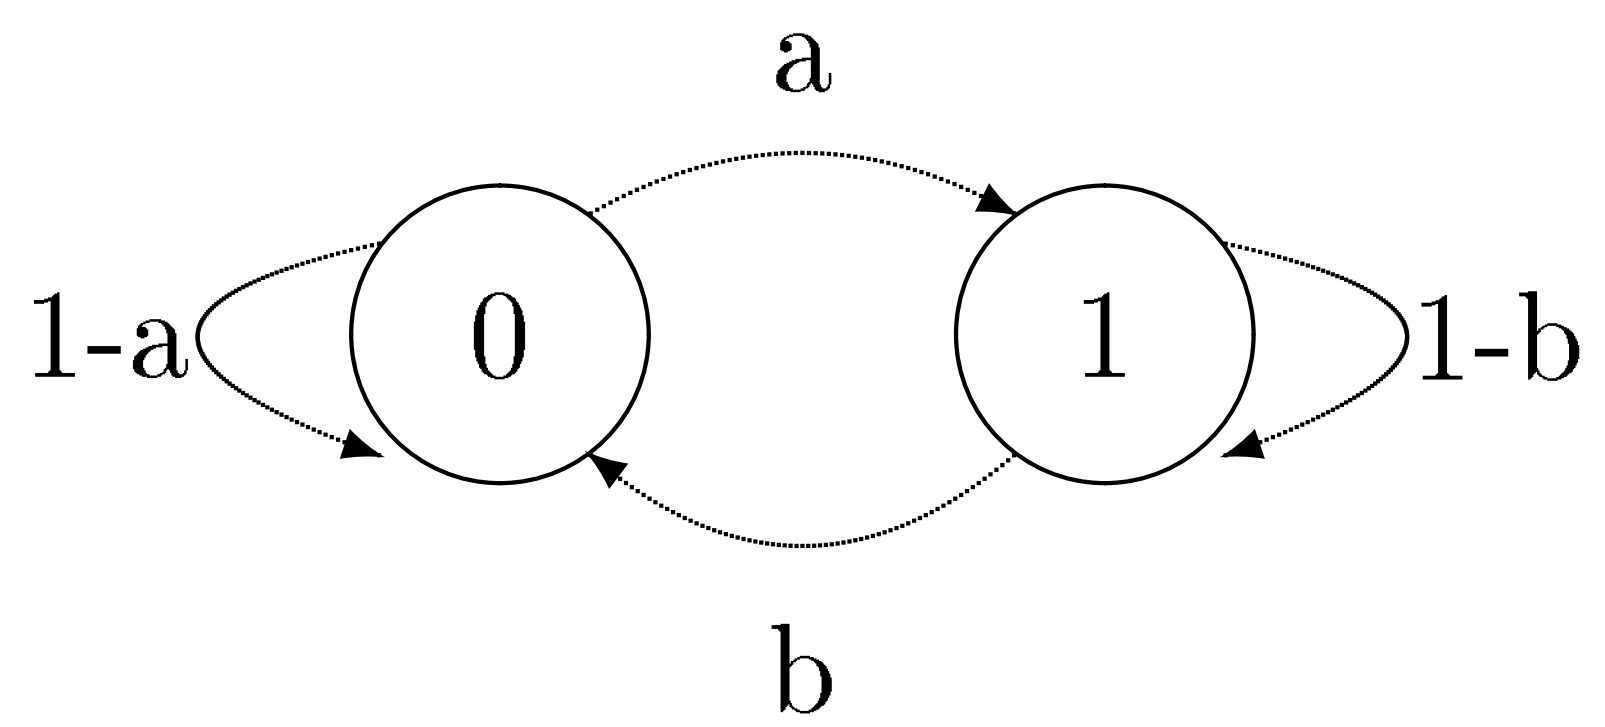
\includegraphics[width=0.8\linewidth]{./Content/Markov/statediag}
\end{minipage}
\begin{minipage}{0.4\textwidth}
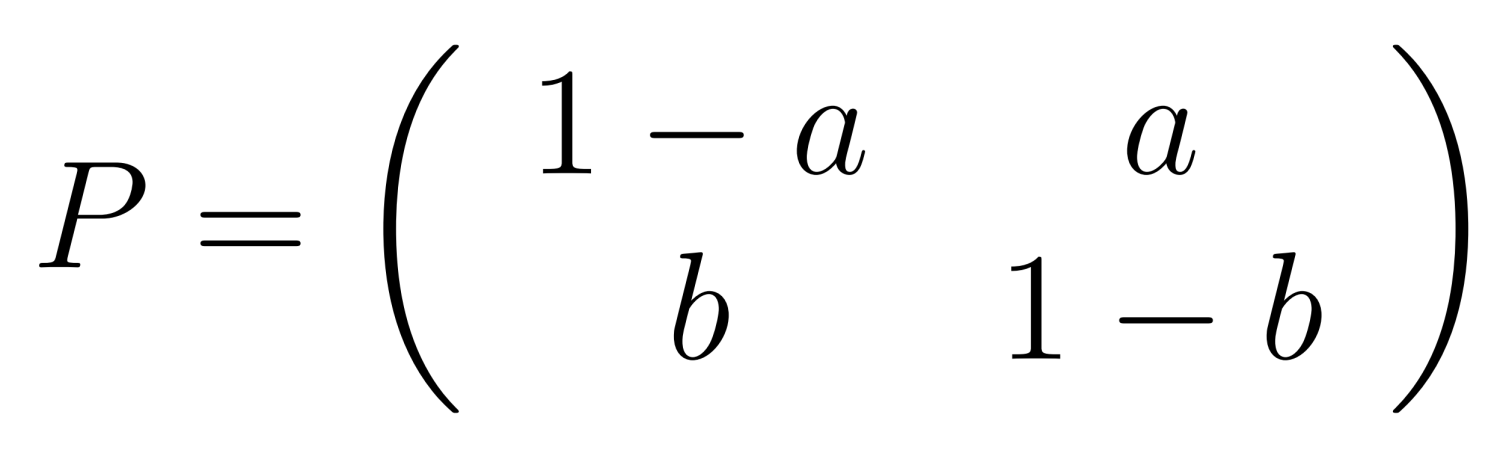
\includegraphics[width=0.8\linewidth]{./Content/Markov/statetab}
\end{minipage}
\hfill


\subsubsection{The Chapmann-Kolmogorov equations \skript{107-108}}
The (exactly) $m$ step transition probabilities of a homogeneous Markov chain $X$ are definde by: 

\begin{equation}
	p_{ij}^{(m)}=P(X_m=j|X_0=i)	\\ 
	p_{ij}^{(n+m)}=\sum\limits_k{p_{ik}^{(n)}p_{kj}^{(m)}}\\
	P^{n+m}=P^nP^m\nonumber
\end{equation}


\subsubsection{The stationary distribution \skript{109}}
The stationary distribution ($n\rightarrow \infty$) of a Chain is:
\begin{equation}
	\boxed{\pi_{j}=\underbrace{\sum\limits_k{\pi_k p_{kj}}}_{\text{probabilities to enter state }j},~~ \pi_j\geq 0 ~~ and ~~ \sum\limits_k{\pi_j}=1}\nonumber
\end{equation}

$\pi$ is a eigenvector of $P$ with eigenvalue $1$\\

The equations below are to solve to get the eigenvector $\pi$:

\begin{equation}
\bm{\pi}=\bm{\pi}\cdot \bm{P}=\begin{pmatrix}\pi_1& \ldots & \pi_n\end{pmatrix}=\begin{pmatrix}\pi_1& \ldots & \pi_n\end{pmatrix}\cdot\begin{pmatrix}
		p_{11} &\cdots & p_{1n}\\
		\vdots& & 	\vdots\\
		p_{n1} &\cdots & p_{nn}\\
	\end{pmatrix}\qquad and\qquad\pi_1+\ldots+\pi_n=1\nonumber
\end{equation}

\begin{itemize}
\item $\pi_i$ is the time (in \%) spent in state $i$
\end{itemize}

The older TI-89 can't solve matrix equation. $\bm \pi$ can be found by calculating 
$\bm P^{100} \approx \bm P^\infty = \begin{bmatrix}\pi_1 & \ldots & \pi_n\\ \vdots &\ddots &\vdots\\\end{bmatrix}$

\subsubsection{Some Definitions \skript{112}}
\begin{itemize}
\item We say a state $j\in S$ is \textbf{accessible} from a fixed state $i\in S$ if there exists $n\geq 0 $ such that $p_{ij}^n>0$. We write $i\rightarrow j$
\item If $j$ is acessible from $i$ and $i$ from $j$, we say that $i$ and $j$ \textbf{communicate} and write $i \leftrightarrow j$
\item $X$ is \textbf{irreducible} if all states communicate with each other. Note that this is equivalent with the existene of a path in the state transition diagram from $i$ to $j$ and back from $j$ to $i$ for all pairs of state $i$, $j$.\\

An irreducible Markov chain has \textbf{only one stationary distribution}.
(Wenn man einen Weg vom ersten Zustand, durch alle anderen Zustände und wieder zurück zum ersten Zustand mit einer Wahrscheinlichkeit ungleich Null findet.)
\end{itemize}

Given a Markov Chain $X$ with state space $S$. For any state we let $f_i$ be the probability of returning to the state $i$ if the chain starts at $i$.

\begin{itemize}
\item We say that a state $i \in S$ is \textbf{recurrent} if $f_i=1$. Hence, with probability $1$ the process will eventually reenter the state $i$. At least one state have to be recurrent. $f_i=P($return to i$|$in i$)$
\item We say that a state $i \in S$ is transient if $f_i<1$. Hence, with strictly positive probability $1-f_i$ the process will never again reenter the state $i$.
\item If state $i$ is recurrent (resp. transient) then all states communicating with $i$ are also recurrent (resp. transient).
\end{itemize}


If the transition matrix P of a Markov chain is such that exists $m \in \mathbb{N}$ with the property that all entries of $P^m$ are strictly positive then:
\begin{itemize}
\item There exists one unique stationary distribution $\pi$
\item For every initial condition $\lim\limits_{n\rightarrow \infty}{\nu(n)}=\lim\limits_{n\rightarrow \infty}{\nu(0)P^n}=\pi$
\item The rows of $P^n$ converge towards the stationary vector $\pi$
\end{itemize}

\vfill

\subsubsection{Random walks on graphs}

\textbf{Definition: } A graph $G$ consists of a vertex set $V$ and a edge set $E$ where each edge is an unordered pair of vertices.

\vspace{0.25cm}

\begin{minipage}{0.15\textwidth}
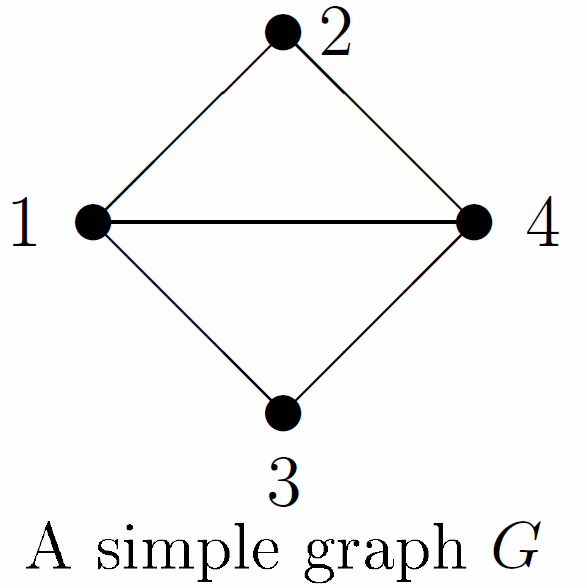
\includegraphics[width=\textwidth,trim= 0cm 2cm 0cm 0cm,clip]{./Content/Markov/simpleGraph}
\end{minipage}
\hfill
\begin{minipage}{0.8\textwidth}
This picture shows a simple-graph $G=(V,E)$ with Vertex set $V=\{1,2,3,4\}$ and edge set $E=\{\{1,2\},\{1,3\},\{1,4\},\{2,4\},\{3,4\}\}$. (Simple graph because no loops and no multiple edges). The multi-graph with loops and multiple edges don't considered here.
\end{minipage}

%\vspace{0.25cm}

\begin{itemize}
	\item \textbf{The degree} $d_i$ of a vertex $i \in V$ is the number of edges incident to the vertex $i$. In the example above it is $d_1=d_4=3$ and $d_2=d_2=2$.
	\item \textbf{The volume} of a subset of vertices $S \subset V$ is \qquad $\text{Vol}(S)=\sum\limits_{i\in S}^{} d_i$
	\item \textbf{A path} from $i$ to $j$ of length $n$ in $G$ is an ordered sequence of distinct vertices $i=v_0,v_1,\ldots,v_n=j$ satisfying $\{v_k,v_{k+1}\} \in E$ for $k=0,1,\ldots,n-1$.
	\item A graph is \textbf{connected} if for any two vertices $i$ and $j$, there is a path from $i$ to $j$.
	\item The \textbf{adjacency matrix} $\bm{A}=(a_{ij})$ pf a simple graph $G$ on $n$ vertices is the $n \times n$  matrix is: $\mtwopartdef{1}{\{i,j\} \in E}{0}$
	\item The \textbf{degree matrix} $\bm{D}$ of a simple graph G on n vertices is the $n \times n$ diagonal matrix $\bm{D}=diag(d_1,\ldots,d_n)$ where $d_i$ is the degree of vertex $i$
	\item The \textbf{transition probabilities} of the random walk on graph G is: $\bm{P}=\bm{D^{-1}A}$ \qquad $p_{ij}=(\bm{P})_{ij}=\mtwopartdef{1/d_i}{\{i,j\} \in E}{0}$
	\item \textbf{Example} for graph G:\\
	\begin{equation}
		\bm{A}=\begin{pmatrix}
			0 & 1 & 1 & 1\\
			1 & 0 & 0 & 1\\
			1 & 0 & 0 & 1\\
			1 & 1 & 1 & 0
		\end{pmatrix}\\
		\bm{D}=\begin{pmatrix}
			3 & 0 & 0 & 0\\
			0 & 2 & 0 & 0\\
			0 & 0 & 2 & 0\\
			0 & 0 & 0 & 3
		\end{pmatrix}\\
		\bm{P}=\begin{pmatrix}
			0 & 1/3 & 1/3 & 1/3\\
			1/2 & 0 & 0 & 1/2\\
			1/2 & 0 & 0 & 1/2\\
			1/3 & 1/3 & 1/3 & 0
		\end{pmatrix}\\
	\end{equation}\nonumber
\end{itemize}

\textbf{Theorem: } Under ergodic conditions we have for \textbf{any initial condition} $\nu: V \rightarrow \mathbb{R}, \sum\limits_{i}^{}{\nu_i=i}$ that the distribution after $k$ steps, $\nu\bm{P}^k$, converges to the unique distribution $\pi$:

\begin{equation}
	\boxed{\lim\limits_{k \rightarrow \infty}{\big(\nu\bm{P}^k\big)_i}=\pi_i=\frac{d_i}{\sum\limits_{j}^{}{d_j}}}\\
	\text{convergence speed:\qquad} ||\nu\bm{P}^2-\pi || \leq \e^{-s\lambda^{'}}\frac{\underset{i}{max}\sqrt{d_i}}{\underset{j}{min}\sqrt{d_j}}\nonumber\\
\end{equation}

with $\lambda^{'}=min\{\lambda_2,2-\lambda_n\}$ where $\lambda_2$ is the second largest and $\lambda_n$ the smallest eigenvalue of $\bm{P}$.\\

\textbf{Example for simple-graph $G$: } 
\todo {Check example}

\renewcommand{\arraystretch}{2.0}
\begin{tabular}{ll}
\textbf{Stationary distribution: }& $\pi_1=\frac{d_1}{\sum\limits_j{d_j}}=\frac{3}{3+2+2+3}=\frac 3 {10} \qquad \pi_2=\frac{d_2}{\sum\limits_j{d_j}}=\frac{2}{3+2+2+3}=\frac 2 {10}  \qquad \pi_3=\frac 2 {10}  \qquad \pi_4=\frac 3 {10}$\\
Eigenvalue: & $|\bm{P}-\lambda\bm{I}|=0\quad \rightarrow \quad \lambda_i\qquad \text{for the example: }\lambda_1=1\quad\lambda_2=0\quad\lambda_3=-1/3\quad\lambda_4=-2/3$\\
Exponent e-function: & $\lambda^{'}=min\{\lambda_2,2-\lambda_n\}=min\{0,2-(-2/3)\}=0$\\
\textbf{Convergence speed: }& $||\nu\bm{P}^2-\pi || \leq \e^{-s\lambda^{'}}\frac{\underset{i}{max}\sqrt{d_i}}{\underset{j}{min}\sqrt{d_j}}=\e^{-s\cdot 0} \frac{\sqrt{3}}{\sqrt{2}}=\frac{\sqrt{3}}{\sqrt{2}}$
\end{tabular}
\renewcommand{\arraystretch}{1.0}













\subsection{Hidden Markov Models (HMM) \skript{122-131 and HMM-Skript}}

\renewcommand{\arraystretch}{1.5}
\begin{tabular}{llll}
Hidden Markov Model& $M$&&\\
Probability of transition from state $i$ to state $j$:&
$P_{ij}=P(X_{t+1}=j|X_t=i)$&&\\
Probability of emitting symbol $j$ in state $i$ :&
$O_{ij}=P(Y_{t}=s_j|X_t=i)$&&\\
Initial probability to be in state $i$:&
$\bm{\pi_i}:=P(X_1=i),i \in S$&&\\
Hidden sequence:&
 $X_t$\quad such as $X_t=\{x_1,x_2,\ldots,x_t\}$&or& $X_{t+1}=\{x_1,x_2,\ldots,x_t,x_{t+1}\}$\\
Observed sequence:&
 $Y_t$\quad ~such as $Y_t=\{y_1,y_2,\ldots,y_t\}$&or& $Y_{t+1}=\{y_1,y_2,\ldots,y_t,y_{t+1}\}$\\
Number of hidden states & $N$&&\\
Time & $1 \leq t \leq T$&&
\end{tabular}

\renewcommand{\arraystretch}{1.0}
\begin{equation}
	\bm{P}=\begin{pmatrix}
		a_{11} & a_{12} & a_{13}\\
		a_{21} & a_{22} & a_{23}\\
		a_{31} & a_{32} & a_{33}
	\end{pmatrix} \quad
	\sum\limits_j a_{ij} = 1\\ 
	\bm{O}=\begin{pmatrix}
		b_{11} & b_{12} & b_{13} & b_{14}\\
		b_{21} & b_{22} & b_{23} & b_{24}\\
		b_{31} & b_{32} & b_{33} & b_{34}\\
	\end{pmatrix} \quad
	\sum\limits_k b_{jk} = 1\\
	\bm{\pi}=\begin{pmatrix}
		\pi_1\\
		\pi_2\\
		\pi_3\\
	\end{pmatrix}\nonumber
\end{equation}

\begin{minipage}{0.3\textwidth}
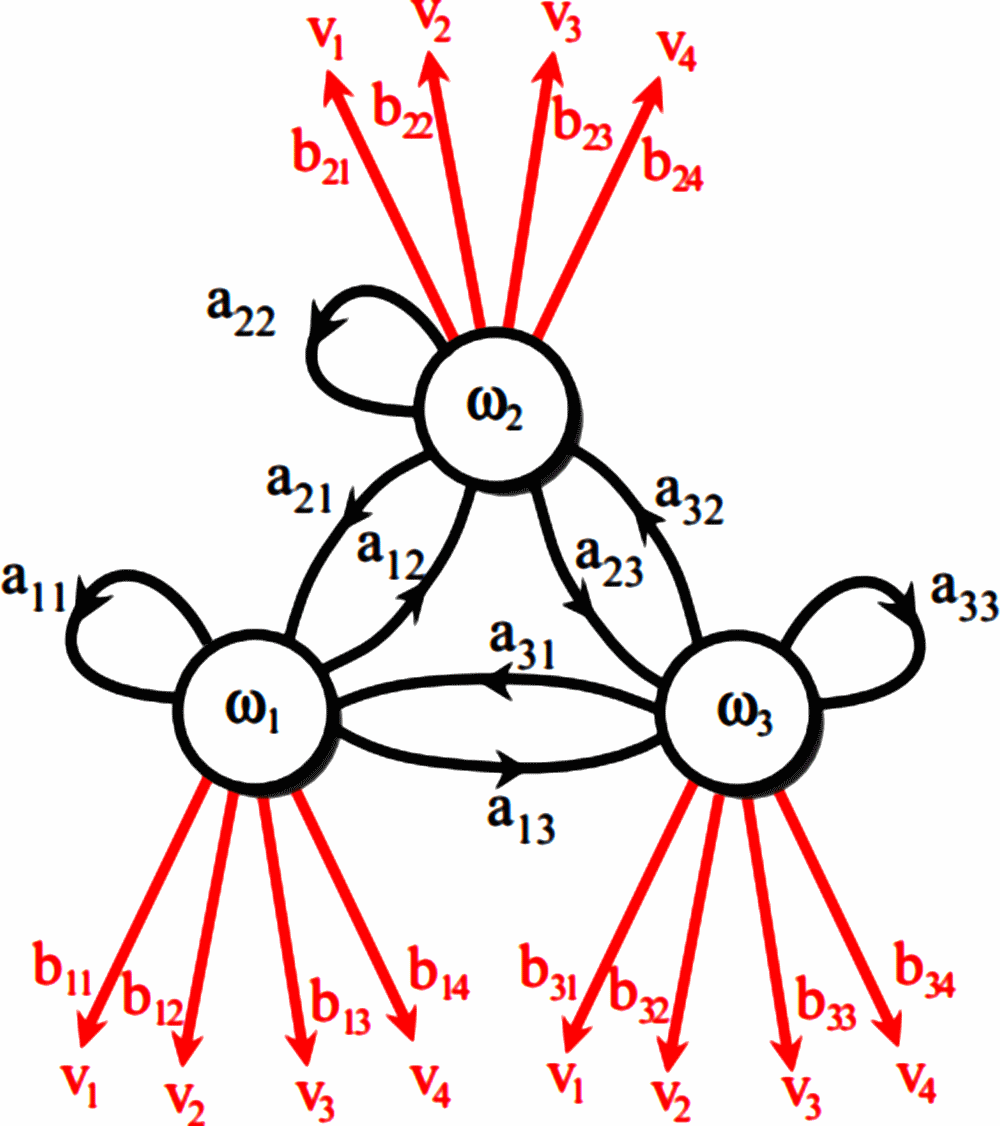
\includegraphics[width=1\linewidth]{./Content/Markov/hiddenMarkovModel.png}
\end{minipage}
\begin{minipage}{0.4\textwidth}
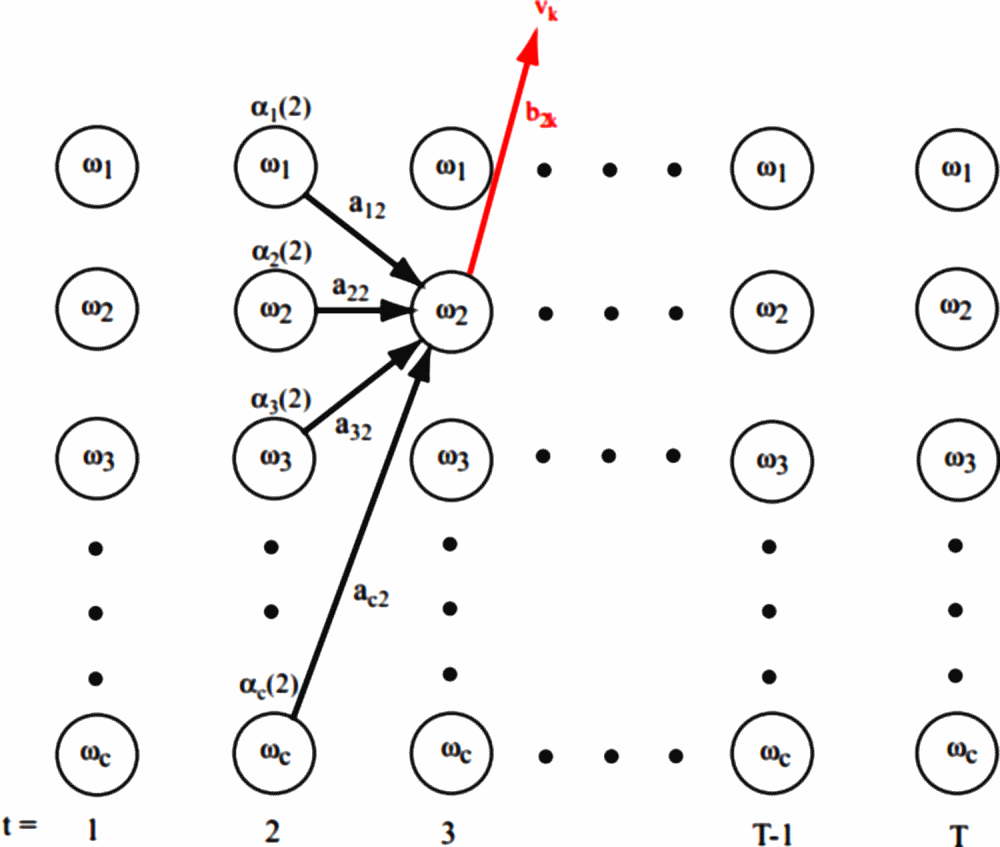
\includegraphics[width=1\linewidth]{./Content/Markov/hiddenMarkovModel2.png}
\end{minipage}
\begin{minipage}{0.3\textwidth}
  \subsection{Problems}
    \begin{liste}
      \item Evaluation problem: Determine the \em probability \em that a particular sequence of 
      visible states $\bm V_T$ was generated by \em that model\em.
      \item Decoding problem: Determine the \em most likely sequence of hidden states \em $\bm \omega^T$ that
      led to observations $\bm V_T$.
      \item Learning problem: Given the structure and training observations, \em learn the parameters \em
      $a_{ij}$ and $b_{jk}$. 
    \end{liste}
\end{minipage}
\vspace{5mm}
\hrule
\vspace{5mm}
\begin{minipage}{0.55\textwidth}
	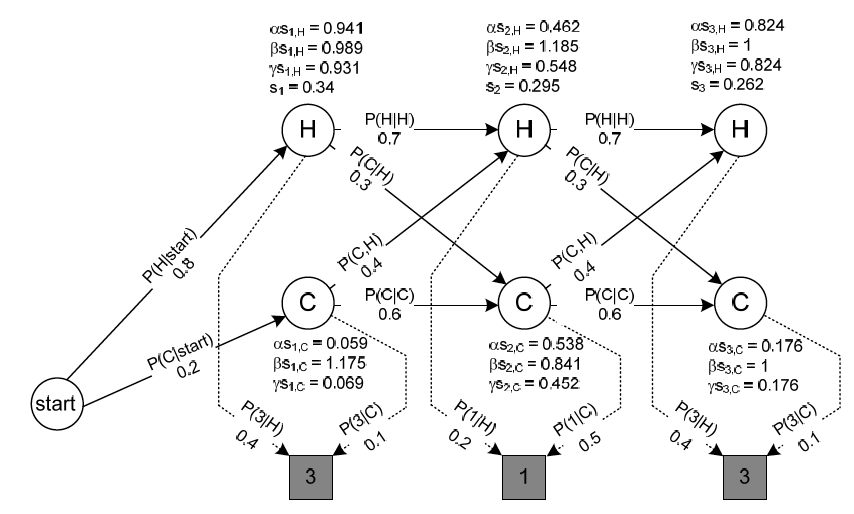
\includegraphics[width=1\linewidth]{./Content/Markov/hmm.png}
\end{minipage}
\begin{minipage}{0.44\textwidth}
	\textbf{Example:}\\
	\begin{tabular}{ll}
											&	Scaled	\\
	$\alpha_{1,H}=P(H|start) P(3|H)$	&	$\alpha S_{1,H}= \displaystyle\frac{\alpha_{1,H}}{\alpha_{1,H}+\alpha_{1,C}} $ \\
	$\alpha_{1,C}=P(C|start) P(3|C)$	&	$\alpha S_{1,C}= \displaystyle\frac{\alpha_{1,C}}{\alpha_{1,H}+\alpha_{1,C}}$ \\
	\end{tabular}
	
	$\alpha_{2,H}=\alpha_{1,H}P(H|H)P(1|H) + \alpha_{1,C}P(C|H)P(1|H)$ \\
	$\alpha_{2,C}=\alpha_{1,H}P(H|C)P(1|C) + \alpha_{1,C}P(C|C)P(1|C)$ \\
	
	$\beta_{1,H}=\beta_{2,H}P(1|H)P(H|H) + \beta_{2,C}P(1|C)P(C|H)$ \\
	$\beta_{1,C}=\beta_{2,C}P(1|C)P(C|C) + \beta_{2,H}P(1|H)P(H|C)$ \\
	
	$\gamma_{1,H}=\alpha_{1,H}\beta_{1,H}$ \\
	$\gamma_{1,C}=\alpha_{1,C}\beta_{1,C}$ \\
 
	 
	
\end{minipage}
\hrule
\vspace{5mm}

\begin{minipage}[t]{0.49\textwidth}

\subsection{Forward Algorithm (Evaluation)}
The forward algorithm can be used to find the probability of an observed sequence $Y_t$.

\begin{aufzaehlung}
	\item Initialization for states $1\leq i \leq N$ at time $t=1$:\\
	
	\vspace{-0.3cm}
	
	$\boxed{\textcolor{blue}{\alpha_1}(i)=\pi_i b_j(y_1)}$ 
	
	\item Recursion for states $1\leq j \leq N$ and time $1\leq t\leq T-1$:\\
		
	\vspace{-0.3cm}
	
  $\boxed{\textcolor{blue}{\alpha_{t+1}}(j)=b_{j}(y_{t+1}) \sum\limits_{i=1}^{N}{\textcolor{blue}{\alpha_t}(i)a_{ij}}}$
	
	\item Total probability for unscaled values\\
		
	\vspace{-0.3cm}
	
	$\boxed{P_{tot} = P(Y_t|M)=\sum\limits_{i=1}^{N}{\textcolor{blue}{\alpha_T(i)}}}$
\end{aufzaehlung}
\end{minipage}
\hfill
\begin{minipage}[t]{0.49\textwidth}
\subsection{Backward Algorithm (Evaluation)}
The backward algorithm is important for the Baum-Welch algorithm. If the target is to find the probability of an observed sequence $Y_t$, then 
the forward algorithm is sufficient. The backward algorithm starts from the last observation and goes backwards.

\begin{aufzaehlung}
	\item Initialization for $1 \leq i \leq N$ at time $t=T$:\\
	
	\vspace{-0.3cm}
	
	$\boxed{\textcolor{blue}{\beta_T}(i)=1}\to$ where $T$ is the last observation time
	\item Recursion for states $1 \leq j \leq N$ and time $2\leq t\leq T$:\\
	
	\vspace{-0.3cm}
	
	 $\boxed{\textcolor{blue}{\beta_{t-1}}(j)=\sum\limits_{i=1}^{N}{b_i(y_t)\textcolor{blue}{\beta_t}(i)a_{ji}}}$
	 \item Conditional probability for the state $x_i$:\\
	 	
	 \vspace{-0.3cm}
	 	
	 $\boxed{P(X_t=x_i|Y_t,M)=\frac{P(X_t=x_i,Y_t|M)}{P(Y_t|M)}=\frac{\textcolor{blue}{\alpha_t}(i)\textcolor{blue}{\beta_t}(i)}{P(Y_t|M)}}$
	 
\end{aufzaehlung}
\end{minipage}

\vspace{1cm}

\begin{minipage}[t]{0.49\textwidth}
\subsection{Viterbi Algorithm (Decoding)}
Be aware, this is not always the same $\alpha$ as in the forward algo (except for $\alpha_1(i)$).
\begin{aufzaehlung}
	\item Initialization for $1\leq i \leq N$:\\
	
	\vspace{-0.3cm}
	
	$\boxed{\textcolor{blue}{\alpha_1}(i)=\pi_i b_j(y_{1})}$
	\item Recursion for $1\leq t\leq T-1$ and $1\leq j \leq N$:\\
			
		\vspace{-0.3cm}
		
		$\boxed{\textcolor{blue}{\alpha_{t+1}}(j)=b_{j}(y_{t+1}) \max\limits_{i \in \{1,\ldots,N\}}{\textcolor{blue}{\alpha_t}(i)a_{ij}}}$
		
		\item Termination: (find the winner state)\\
			
		\vspace{-0.3cm}
		
		$\boxed{P(X_t|Y_t)=\max\limits_{j \in \{1,\ldots,N\}}{\textcolor{blue}{\alpha_T}(j)}}$
	\item Backtracking (All the stored way back):\\
				
		\vspace{-0.3cm}
			
		$\boxed{X_t=\arg~ \underset{j \in \{1,\ldots,N\}}{\max}~{\textcolor{blue}{\alpha_T}(j)}}$\\
		Starting from the biggest argument of $\alpha_T$ go backwards through the edges with the highest probability.
\end{aufzaehlung}	 
\end{minipage}
\hfill
\begin{minipage}[t]{0.49\textwidth}

\subsection{Baum-Welch Algorithm (Learning)}

\begin{aufzaehlung}
	\item Initialization for $1\leq i \leq N$:\\
	
	\vspace{-0.3cm}
	
	Assign arbitrary model parameters\\

	\item Iteration:\\
			
	\vspace{-0.3cm}
	
	Set $\bm{A_{kl}}$ and $\bm{B_{k}(x)}$ to a pseudocount value.\\
	
	FOR  each training data set $\bm{X}^m$:\\
	
	\qquad Forward algoritm: $\textcolor{blue}{\alpha_t}(i)$
	
	\qquad Backward algoritm: $\textcolor{blue}{\beta_t}(i)$
	
	\qquad Add contributions to $\bm{A_{kl}}$ and $\bm{B_{k}(x)}$
	
	\qquad Update $a_{ij}=\frac{A_{ij}}{\sum\limits_{k}^{}{A_{ik}}}$ and $b_k(x)=\frac{B_k(x)}{\sum\limits_{l}^{}{B_{k}(l)}}$
	
	\item Termination:\\
		
	UNTIL stop criterion reached
		
\end{aufzaehlung}	 
\end{minipage}

\subsection{Some properties}
\begin{itemize}
	\item The $\gamma$-Value: $\boxed{\gamma_t(j)=\textcolor{blue}{\alpha_t}(j)\cdot\textcolor{blue}{\beta_t}(j)}$
	\item A property of the $\gamma$-Value: is: $\boxed{\sum\limits_{j=1}^{N}{\gamma_t(j)=P_{tot}}}$ \\  
	$\to$ Example: $P_{tot}=\gamma_2(Hot)+\gamma_2(Cold)=\alpha_2(Hot)\cdot\beta_2(Hot)+\alpha_2(Cold)\cdot\beta_2(Cold)$
	\item Probability that the state was $x$ at time $t$ given the sequence $Y_t$: $\boxed{P(X_t=x|Y_t)=\frac{\textcolor{blue}{\alpha_t}(x)}{\sum\limits_{j=1}^{N}{\textcolor{blue}{\alpha_t}(j)}}}$
\end{itemize}





\newpage

\section{Continuous-time Markov Chains \skript{131-148}}

\subsubsection{Exponential RV $X\sim Exp(\lambda)$ (Recall) \skript{131}}
The main reason why the exponential distribution comes in naturally in Markov processes is \textbf{the memoryless property}: 
$$P[X>s+t|X>t]=P[X>s] \text{ for all } s,t\geq 0$$
\textbf{Proof: }$P[X>s+t|X>t]=\frac{P[X>s+t,X>t]}{P[X>t]}=\frac{P[X>s+t]}{P[X>t]}=\frac{\e^{-\lambda(s+t)}}{\e^{-\lambda t}}=\e^{-\lambda s}=P[X>s]$

\begin{minipage}{0.7\textwidth}
\begin{equation}
f_X(x) = \twopartdef { \lambda\e^{-\lambda x} } {x\geq 0} {0} {x<0}\\
F_X(x) = \twopartdef { 1-\e^{-\lambda x} } {x\geq 0} {0} {x<0}\nonumber
\end{equation}
\end{minipage}
\begin{minipage}{0.3\textwidth}
	\begin{itemize}
		\item $E(X)=\frac {1}{\lambda}$
		\item $Var(X)=\frac {1}{\lambda^2}$
		\item $\phi(t)=\frac{\lambda}{\lambda-t}$
	\end{itemize}
\end{minipage}
\hfill

\subsubsection{Some relations \skript{133-134}}
A time continuous stochastic process $X$ with countable state space $S$ is a continuous-time Markov chain if: 

$$P\big(X(t+s)=j\big|X(s)=i,X(u)=x_u,0\leq u\leq s\big)=P\big(X(t+s)=j\big|X(s)=i\big) \quad\text{for all } s,t\geq 0 \text{ and all } i,j,x_i\in S$$

\begin{itemize}
	\item For ease of presentation we will suppose, save indication to the contrary, that from now on $S=\{0,1,2,\ldots\}$.
	\item We assume that the markov chains have time-homogeneous transition probabilities: $$p_{ij}(t,s):=P\big(X(t+s)=j|X(s)=i\big)=p_{ij}(t)$$
	\item $p_{ij}(t)$ is called the transition function of the time-homogeneous process.
	\item $\sum\limits_{j\in S}^{}{p_{ij}(t)=1}$ for all $i \in S$
	\item Let $\tau_i$ be the time that the process spends in state $i$ befor making a transition to some other state. We may write that.
	$$P\big[\tau_i>s+t\big|\tau_i>t\big]=P\big[\tau_i>s\big] \quad\text{for all } s,t\geq 0$$
	Since the process is Markovian, the time it has to spent in a given state does not influence the future. Consequently, whatever the time that the process has already spent in $i$, it is as likely that it will remain there during at least $s$ additional time units that if it had just entered this state. Since we have the memoryless property, we can conclude that $\tau_i$ has an exponential distribution with parameter $\nu_i$, depending on state $i$:
	$$\tau_i\sim Exp(\nu_i)$$
	Moreover, the Markov property also implies that the next state visited $j$, is independent pf $\tau_i$
	$$p_{ij}\geq 0, \quad p_{ii}=0, \quad \sum\limits_{j\in S}^{}{p_{ij}(t)}=1\quad \text{for all } i \in S$$
	
\end{itemize}

\subsubsection{The  Chapmann-Kolmogorov equations \skript{136}}

$$p_{ij}(t+s)=\sum\limits_k{p_{ik}(t)p_{kj}(s)}=\sum\limits_k{p_{ik}(s)p_{kj}(t)}\quad\text{for all } s,t\geq 0 \quad\text{and } i,j\in S$$

\textbf{Notation:} $p_j(t)=P(X_t=j)$ \qquad If the initial distribution is given by $a_i=P(X_0=i)$ then\quad $p_j(t)=\sum\limits_{i=0}^{\infty}{a_i p_{ij}(t)}$

%\todo{Skript:137 dazunehmen?}

\subsubsection{Counting processes \skript{139}}

A stochastic process $\{N_t,t\geq 0\}$ is said to be a counting process if $N_t$ represents the total number of events that occur by time $t$.

\textbf{Properties:}

\begin{itemize}
\item $N_t\geq 0$ and $N_t \in \mathbb{Z}$ (integer valued)
\item If $s<t$ then $N_s\leq N_t$
\item $N_t-N_s$ equals the number of events that occur in the interval $(s,t]$
\end{itemize}

\subsubsection{The Poisson process \skript{139}}

One of the most important counting process is the Poisson process which \textbf{definition} is:

\begin{aufzaehlung}
	\item $N_0=0$
	\item The process has independent increments: $N_{t4}-N_{t3}$ and $N_{t2}-N_{t1}$ are independent for all $t_1<t_2\leq t_3<t_4$.
	\item The number of events in any interval of length $t$ is Poisson distributed with mean $\lambda t$. That is for all $s,t\geq 0$
	
	\begin{minipage}{11cm}
		$$\boxed{P\big(N_{t+s}-N_s=n\big)=\e^{-\lambda t}\frac{(\lambda t)^n}{n!}\quad n=0,1,2,\ldots \quad n= \text{ nr. of events}}$$
		\begin{center}
		\textbf{Example of a Poisson process:}\\
			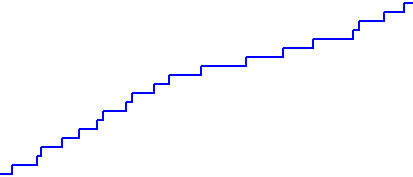
\includegraphics[width=6cm]{Content/Markov/SampleProcessPoisson}
		\end{center}	
	\end{minipage}
	\hfill
	\begin{minipage}{8cm}
		\begin{itemize}
			\item $E(N_t)=\lambda t$
			\item $Var(N_t)=E(N_t^2)-E(N_t)^2=\lambda t$
			\item $\phi(t)=\e^{\lambda t(\e^t-1)}$
			\item $R_N(t,t+s)=\lambda^2 t(t+s)+\lambda t$
			\item $C_N(t_1,t_2)=\lambda\min(t_1,t_2)$
		\end{itemize}
	\end{minipage}
%	\item \todo{Definition 24 auch? (Die sind angeblich gleich wie Definition 23 (Siehe Seite 143))}
	%\item for small $h\geq 0$ we have $P\big(N_h=1\big)=\lambda h +o(h)$ 	\todo{what???}
	%\item for small $h\geq 0$ we have $P\big(N_h\geq 2\big)=o(h)$			\todo{what???}
	\item Given a sequence $\{\tau_n,n\geq 1\}$ of independently and identically distributed exponential random variables.
	
	\begin{minipage}{11.25cm}
	Each having parameter $\lambda$. Define the counting process $\{N_t\geq 0\}$ by the expression:
	$$N_t=max\{n|S_n\leq t \}$$
	
	where $S_n:=\tau_1+\tau_2+\ldots+t_n$ is the time at which the n'th event occurs.
	The counting process $N_t$ is a Poisson process having rate $\lambda>0$.
	$S_n$ is the arrival time of the $n$th event and follows an Erlang$(n,\lambda)$ distribution. It is easy to see that $N_t\geq n \Leftrightarrow S_n\leq t$ (figure right)
	\end{minipage}
	\hfill
	\begin{minipage}{6.25cm}
	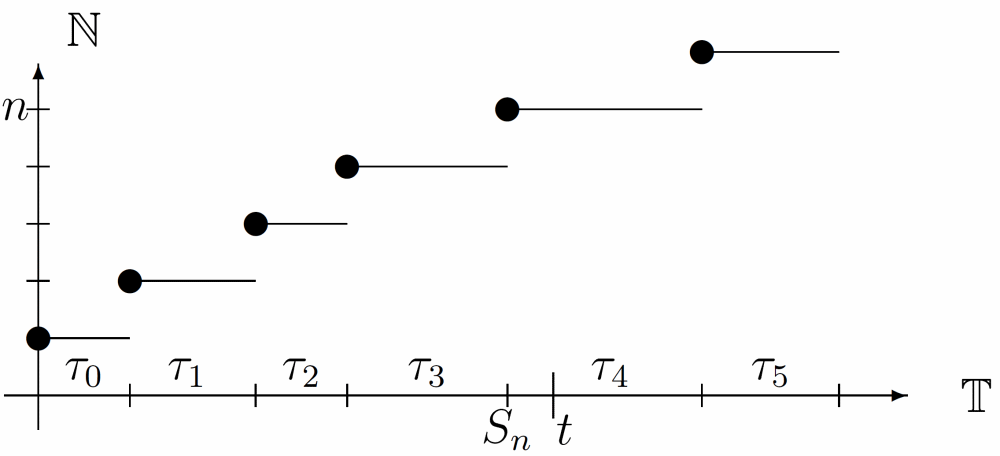
\includegraphics[width=\textwidth]{Content/Markov/erlang}
	\end{minipage}
\end{aufzaehlung}


\begin{minipage}[t]{6.5cm}
\textbf{Generating matrix $G$}:
$$G=\begin{pmatrix}
-\lambda & \lambda & 0 & 0 &\ldots\\
0&-\lambda & \lambda & 0  &\ldots\\
0 & 0&-\lambda & \lambda & \ldots\\
\vdots&\vdots&\vdots&\vdots&\ddots\\
\end{pmatrix}$$

\vspace{0.25cm}

\textbf{Memoryless Expectation $E(\tau)$}:
$$E(\tau|\tau>s)=s+E(\tau)=s+\frac 1\lambda$$

\end{minipage}
\hfill
\begin{minipage}[t]{12.5cm}
\textbf{(Inter)arrival time $\tau$}:
\begin{itemize}
\item (Inter)arrival time: $\tau~Exp(\lambda)$ between two sequentially events:
\item Probability that the (inter)arrival time between two sequentially events is bigger then $s$:\\
 $P(\tau>s)=\int\limits_{s}^{\infty}{\lambda\e^{-\lambda t}dt}=\left[\e^{-\lambda t}\right]_\infty^s=\e^{-\lambda s}$
\item Probability that the (inter)arrival time between two sequentially events is smaller then $s$:\\
 $P(\tau<s)=\int\limits_{0}^{s}{\lambda\e^{-\lambda t}dt}=\left[-\e^{-\lambda t}\right]_0^s=1-\e^{-\lambda s}$
\end{itemize}
\end{minipage}

\renewcommand{\arraystretch}{2}
\begin{tabular}{|l|l|}
	\hline
	\textbf{Two independent Poisson processes with $\lambda_1,\lambda_2$}: & $P(\tau_1 < \tau_2)=\displaystyle\frac{\lambda_1}{\lambda_1+\lambda_2}$ \\
	\textbf{Splitting Poisson process}: & $\lambda_1 = \lambda p \quad \lambda_2 = \lambda (1-p)$\\
	\textbf{Merging two Poisson processes}: & $\lambda = \lambda_1 + \lambda_2$\\
	\hline
\end{tabular}\\
\renewcommand{\arraystretch}{1.0}

\textbf{Examples for some Poisson processes}: 
\begin{itemize}
	\item The total number of persons who enter a particular store
	\item The number of visits of a particular web site
	\item The number of occurrences of earth quakes
	\item The number of occurrences of failure of a given production facility
	\item The number of incoming phone calls in a phone center
	\item The number of electron emission on top of a heated cathode
\end{itemize}

\subsubsection{Birth and death process \skript{145}}

The Poisson process will generalized in a way that allowed the counting process to decrease. Such a process is coined a birth death process. A possible interpretation is the number of clients in a post office where clients enter with exponential arrival times of intensity $\lambda$ and where clients leave the office at an exponential rate $\mu_n$. $n$ is the number of clients in the System.\\

\textbf{Definition of transition rate}: $\nu_{ij}=0 \quad if\quad |j-1|>1$\\

The parameter $\lambda_i:=\nu_{ii+1}$ for $i\geq 0$ and $\mu_i:=\nu{ii-1}$ for $i\geq 1$ are the \textbf{birth rates} and the \textbf{death rates} of the process.

\subsubsection{Limiting probabilities \skript{146}}
$$\pi_j=\lim\limits_{n\rightarrow \infty}{p_{ij}(t)}$$
Under ergodic conditions the limit $\pi_j$ exists for all $j \in\{0,1,\ldots\}$ and can be computed by the following \textbf{balance equations} plus probability normalization:
$$\boxed{\underbrace{\pi_j\nu_j}_{\text{outgoing}}=\underbrace{\sum\limits_{i\neq j}{\pi_i \nu_{ij}}}_{\text{incoming}}\quad \text{for all} \quad j\in\{0,1,\ldots \}
\qquad \qquad \sum\limits_{j=0}^{\infty}{\pi_j=1}}$$

\textbf{Interpretation: }\\
Rate at which the process leaves state $j$: $\nu_j\pi_j$\\
Rate at which the process enters state $j$: $\sum\limits_{i\neq j}{\pi_i \nu_{ij}}$

\textbf{Example for Queuing with a single server}\\
\begin{minipage}{10.5cm}
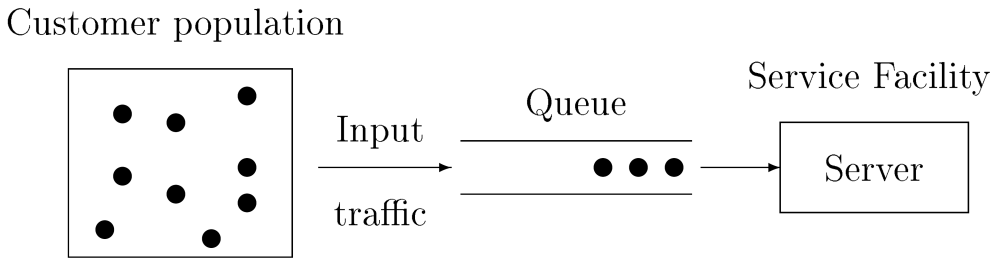
\includegraphics[width=0.8\textwidth]{Content/Markov/Queue.png}
\end{minipage}
\hfill
\begin{minipage}{7.5cm}
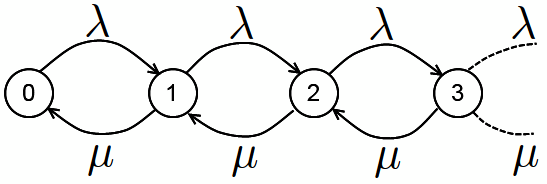
\includegraphics[width=0.8\textwidth]{Content/Markov/queieingGraph.png}
\end{minipage}

\begin{minipage}{5.5cm}
	\textbf{Balance Equation:}
	\begin{align}
		\underbrace{\lambda\pi_0}_{\text{outbound}}			&=\underbrace{\mu\pi_1}_{\text{inbound}}						\nonumber\\[0.25cm]
		(\lambda+\mu)\pi_1		&=\lambda\pi_0+\mu\pi_2	\nonumber\\[0.25cm]
		(\lambda+\mu)\pi_2		&=\lambda\pi_1+\mu\pi_3	\nonumber\\[0.25cm]
		\vdots\qquad			&=\qquad\vdots							\nonumber\\[0.25cm]
		(\lambda+\mu)\pi_{n-1}	&=\lambda\pi_{n-2}+\mu\pi_{n}	\nonumber\\[0.25cm]
		\pi_0+\pi_1+\pi_2&+\ldots+\pi_n=1\nonumber
	\end{align}
\end{minipage}
\hfill
\begin{minipage}{13.5cm}
	\begin{align}
		&\pi_0=\frac{1}{1+\sum\limits_{i=1}^{\infty}{\left(\lambda/\mu\right)^i}}\overset{\frac{\lambda}{\mu}<1}{=}\frac{1}{1+\frac{1}{1-\lambda/\mu-1}}=1-\frac\lambda\mu\nonumber\\[0.25cm]
		&\pi_n=\pi_0\left(\frac{\lambda}{\mu}\right)^n=\left(1-\frac{\lambda}{\mu}\right)\left(\frac\lambda\mu\right)^n\nonumber\\[0.5cm]
		%&\textbf{Total time: }E(X_t)=\todo{???}\nonumber\\[0.5cm]
		&\textbf{Service time: }E(T)=\frac{E(X_t)}{\lambda}\nonumber\\ %\todo{???}\nonumber\\[0.5cm]
		&\textbf{Expected number of clients: }M=\sum\limits_{n=0}^{\infty}{n\pi_n}\nonumber\\
		&\textbf{Use the normalisation: } P\big(n>2\big)=1-\pi_0-\pi_1\nonumber
	\end{align}
\end{minipage}

\vfill



 


\section{Reihenentwicklungen}
\begin{alignat}{4}
&\sum\limits_{k=0}^{n}{\frac{1}{k!}}&&= 1+\frac{1}{1!}+\frac{1}{2!}+\frac{1}{3!}\ldots+\frac{1}{n!} \quad&&\overset{n\rightarrow\infty}{\longrightarrow}\quad \e\nonumber\\[0.1cm]
&\sum\limits_{k=0}^{n}{(-1)^{k}\frac{1}{k!}}&&= 1-\frac{1}{1!}+\frac{1}{2!}-\frac{1}{3!}+\ldots\pm\frac{1}{n!}\qquad&&\overset{n\rightarrow\infty}{\longrightarrow}\quad  \frac1\e\nonumber\\[0.0cm]
&\sum\limits_{k=0}^{n}{(-1)^{k}\frac{1}{k}}&&= 1-\frac{1}{2}+\frac{1}{3}-\frac{1}{4}+\ldots\pm\frac{1}{n}\qquad&&\overset{n\rightarrow\infty}{\longrightarrow}\quad \ln (2)\nonumber\\[0.0cm]
&\sum\limits_{k=0}^{n}{\frac{1}{2^k}}&&= 1+\frac{1}{2^1}+\frac{1}{2^2}-\frac{1}{2^3}+\ldots+\frac{1}{2^n}\qquad&&\overset{n\rightarrow\infty}{\longrightarrow}\quad 2\nonumber\\[0.0cm]
%&\sum\limits_{k=0}^{n}{(-1)^{k}\frac{1}{2^k}}&&= 1-\frac{1}{2^1}+\frac{1}{2^2}-\frac{1}{2^3}+\ldots\pm\frac{1}{2^n}\qquad&&\overset{n\rightarrow\infty}{\longrightarrow}\quad  \frac23\nonumber\\[0.0cm]
&\sum\limits_{k=0}^{n}{\frac{1}{k(k+1)}}&&= \frac{1}{1\cdot2}+\frac{1}{2\cdot3}+\frac{1}{3\cdot4}+\ldots+\frac{1}{n(n+1)}\qquad&&\overset{n\rightarrow\infty}{\longrightarrow}\quad 1\nonumber\\[0.0cm]
&\sum\limits_{k=0}^{n}{\frac{1}{(2k-1)(2k+1)}}&&= \frac{1}{1\cdot3}+\frac{1}{3\cdot5}+\frac{1}{5\cdot7}+\ldots+\frac{1}{(2n-1)(2n+1)}\qquad&&\overset{n\rightarrow\infty}{\longrightarrow}\quad \frac 12\nonumber\\[0.0cm]
&\sum\limits_{k=0}^{n}{\frac{1}{(k-1)(k+1)}}&&= \frac{1}{1\cdot3}+\frac{1}{2\cdot4}+\frac{1}{3\cdot5}+\ldots+\frac{1}{(n-1)(n+1)}\qquad&&\overset{n\rightarrow\infty}{\longrightarrow}\quad \frac 34\nonumber\\[0.0cm]
&\sum\limits_{k=0}^{n}{\frac{1}{k(k+1)(k+2)}}&&= \frac{1}{1\cdot2\cdot3}+\frac{1}{2\cdot3\cdot4}+\ldots+\frac{1}{n(n+1)(n+2)}\qquad&&\overset{n\rightarrow\infty}{\longrightarrow}\quad \frac 14\nonumber\\[0.0cm]
&\sum\limits_{k=0}^{n}{q^k}&&= q+q^2+q^3+\ldots+q^n\qquad&&\overset{n\rightarrow\infty}{\longrightarrow}\quad \frac{1}{1-q}\qquad&& 0\leq q<1\nonumber\\[0.0cm]
&\sum\limits_{k=1}^{n}{q^k}&&= q^2+q^3+q^4\ldots+q^n\qquad&&\overset{n\rightarrow\infty}{\longrightarrow}\quad  \frac{1}{1-q}-1\qquad&& 0\leq q<1\nonumber\\[0.0cm]
&\sum\limits_{k=0}^{n}{\binom{\alpha}{k}x^k}&&\qquad&&\overset{n\rightarrow\infty}{\longrightarrow}\quad  (1+x)^\alpha\qquad&& 0\leq x<1\nonumber\\
&\sum\limits_{k=0}^{n}{k\alpha^k}&&=\alpha+ 2\alpha^2+3\alpha^3\qquad+\ldots+n\alpha^n&&\overset{n\rightarrow\infty}{\longrightarrow}\quad  \frac{\alpha}{\left(1-\alpha\right)^2}\qquad&& 0\leq \alpha<1\nonumber
\end{alignat}

\vfill

%\input{../StatDig/files/WTheorie.tex}
%\section{Ableitungstabelle}
%\begin{center}
%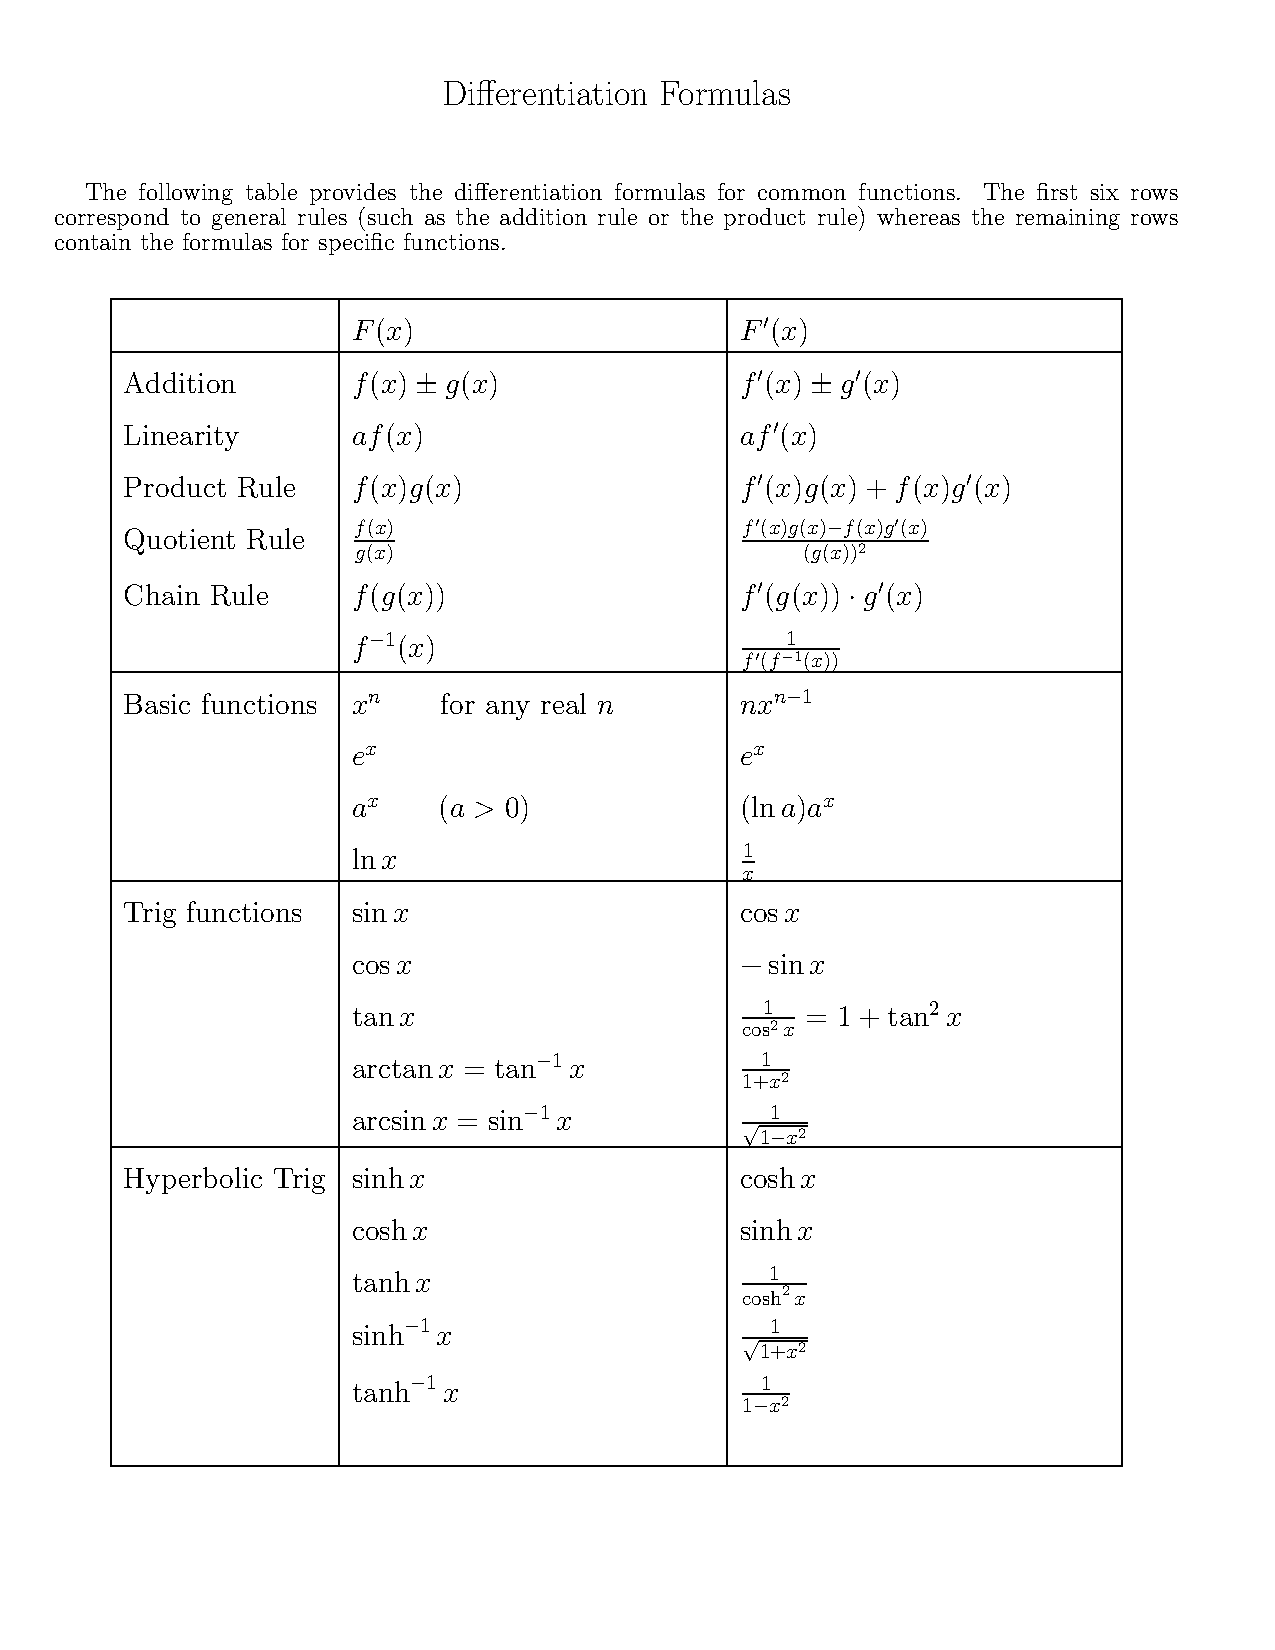
\includegraphics[page=1,width=14cm,trim=1.75cm 3.0cm 2.5cm 5.0cm,clip]{Content/Tabellen/calcrulz.pdf}
%\end{center}
%\hfill
%\newpage
\section{Integration table}

\begin{center}
\includegraphics[page=2,width=18cm,trim=1.25cm 3cm 4.5cm 4cm,clip]{Content/Tabellen/calcrulz.pdf}
\end{center}

\vfill

\section{Übungsverzeichnis}
\begin{tabular}{|l |p{4cm} |p{9.5cm}| l|}
	\hline
	Example 15 	&	$SNR=\frac{E(X^2)}{E(N^2)}$	&	SNR und Schätzer zusammen.				& \skript{37-38} \\
	\hline
	Exercise 22	&								&	Show that if $X$ and $Y$ are independet normal random variables,
													then $X+Y$ is normal with mean $\mu_1+\mu_2$ and variance $\sigma_1^2+\sigma_2^2$.	& \skript{43} \\
	\hline
	Example 17	&								&	Bivariate normal distribution		& \skript{43} \\
	\hline	
	Example 19	&	Law of large numbers		&	Monte-Carlo simulation					& \skript{47} \\
 	\hline
 	Exercise 23	&	Law of large numbers		&	Monte-Carlo simulation, estimate $\pi$	& \skript{48} \\
 	\hline
 	Example 20	&	Central limit theorem		&	Lifetime of battery with std. deviation & \skript{50} \\
 	\hline
 	Example 21	&	Joint probability			&											& \skript{51} \\
 	\hline
 	Example 22	&	Joint probability			&	$n$ components with $X_i\begin{cases}1, \ldots\\0, \text{otherwise} \end{cases}$	& \skript{52}	\\
	\hline
	Exercise 24	&	Conditional probabilities	&	Optical Channel, Poisson distribution	& \skript{52} \\
	\hline
	Exercise 25 &	Conditional probabilities	&	Binary Channel, Bernoulli RV			& \skript{53} \\
	\hline
	Exercise 26	&	Conditional probabilities	& Binary channel receiver design (maximum a posteriori, likelihood ratio). Show that.			& \skript{53} \\
	\hline
	Exercise 27	&	Conditional probabilities	&	Post office, Poisson distribution		& \skript{54} \\
	\hline
	Example	23	&	Joint density of $X$ and $Y$	&										& \skript{55} \\
	\hline
	Example 24	&	Joint density of $X_1$ and $X_2$	&	$\to$ bivariate normal			& \skript{55} \\
	\hline
	Example 25	&	Joint density				&	Gauss-Channel, error probability		& \skript{56} \\
	\hline
	Example 26	&	Joint density				&	Joint density of $X$ and $Y$			& \skript{57} \\
	\hline
	Example 27  & Best selection problem & Finding a flat with learning phase and immediate decision  & \skript{57-58} \\
	\hline
	Example 28	&	A static estimation problem	&	Signal in additive noise $Y=X+N$	& \skript{60} \\
	\hline
	Exercise 28	&	A static estimation problem	&	Signal in additive noise $Y=X+N,$ 
													$X \sim N(0,\sigma_x^2), N \sim N(0,\sigma_N^2)$ 	& \skript{60-61} \\
	\hline
	Example 29	&	Stochastic processes		& Introduction, Sending bits over a noisy channel & \skript{66-68}\\
	\ldots		& & & \\
	Example 34	& & & \\
	\hline	
	Example 35	& 	Stochastic process 			& Random walk with independent Bernoulli random variables & \skript{69} \\
	\hline
	Example 36	&	Stochastic process			& Autocorrelation, autocovariation\ldots Bernoulli &	\skript{72} \\
	\hline
	Example 37	&	Stochastic process			& Random walk, binomial distribution, (mean, autocorrelation, autocovariance)	& \skript{73} \\
	\hline
	Exercise 32	&	Stochastic process			& Prove that if $X$ is strict sens stationary then $X$ is also WSS.	& \skript{75} \\
	\hline
	Exercise 33 &	Stochastic process			& Prove that $Var(X_t)=C_X(0)$ in WSS case.							& \skript{75} \\
	\hline
	Exercise 34	&	Stochastic process			& Prove that $\rho_X(t_1,t_2)=\frac{C_X(t_2-t_1)}{C_X(0)}$ in WSS case.	& \skript{75} \\
	\hline
	Example 41	&	Power spectral density		& Introduction														& \skript{79} \\
	Example 42	&	& & \\ 
	\hline
	Exercise 36	&	Power spectral density		& Show that $R_X(t)=cos(2\pi f t)/2 \FT S_X(k)=2\pi [\delta(k-2\pi f)+ \delta(k+2\pi f)]/4$ &	\skript{80} \\
	\hline
	Example 44	&	Power spectral density		& WSS process through a linear system $\to$ filter.				& \skript{82} \\
	\hline
	Example 45	&	Power spectral density		& Low-pass RC filter		& \skript{84} \\
	\hline
	Example 46	&   Gaussian White Noise		& 	Suppose we describe a particle with mass $m$ moving along the $x$ axis and
													subject to a friction foce proportional to speed.				& \skript{86} \\
	\hline
	Example 66	&	Kalman filter				&	scalar problem	& \skript{171} \\
	\hline
	Exercise 39 & Colored Noise            & Production with failure rate & \skript{97} \\
	\hline
	\ldots \\
	\hline
	Exercise 50	&	Continuous-time Markov chains &	Lifetime exponential distribution $P[L>2/\lambda|L>1/\lambda]$	& \skript{131} \\
	\hline
	Example 61	&								& Let $X \sim Exp(\lambda_1)$ and $Y \sim Exp(\lambda_1)$ independent random variables 
													  $\to P[X<Y]=\displaystyle\int_{0}^{\infty} F_X(y)f_Y(y)dy$	& \skript{131} \\
	\hline
\end{tabular}
\begin{tabular}{|l |p{4cm} |p{9.5cm}| l|}	
	\hline
	Example 63	&	Kolmogorov Equation			& 																	& \skript{136} \\
	\hline
	Exercise 53 &	Poisson process				& Cars on a lane $\to$ a) probability to wait, b) mean length c) mean number & \skript{141} \\
	\hline
	Exercise 54	&								& Merging of two Poisson processes gives a process with $\lambda = \lambda_1+\lambda_2$ & \skript{142} \\
	\hline
	Exercise 55 &								& Splitting of two Poisson processes $\to$ $\lambda_0=(1-p)\lambda \quad \lambda_1=p\lambda$ & \skript{142} \\
	\hline
	Exam 2008.1 &	Binary channel				& Noisy channel, calculate error probability under the majory vote rule & Exam 2008.1 \\
	\hline
	Exam 2008.3 &	Queuing system				& FIFO queuing system with single server & Exam 2008.3	\\
	\hline
	Exam 2009.1 &	Static estimation problem	& Static estimation problem for normal variables & Exam 2009.1 \\
	\hline
	Exam 2009.3 &	Queuing system				& FIFO Queuing system with two server plus one server & Exam 2009.3 \\
	\hline
	Exam 2010.1 &	Disease probability			& Calculate expectation and standard deviation & Exam 2010.1 \\
	\hline
	Exam 2010.3 &	Queuing system				& Queuing system with two server and two types of clients & Exam 2010.3 \\
	\hline
	Exam 2011.1 &	Gauss channel				& Signal with additive noise $Y=X+N$, error probability & Exam 2011.1 \\
	\hline
	Exam 2011.3 &	Queuing system				& Queuing system with two server and two types of clients & Exam 2011.3 \\
	\hline
	Exam 2012.1 &	Proba review				& Sequence of Bernoulli random variables, $E(Y_1)$, $V(Y_1)$, $\rho(Y_1, Y_2)$ & Exam 2012.1 \\
	\hline
	Exam 2012.3 &	Queuing system				& Queuing system with three server and limited capacity & Exam 2012.3 \\
	\hline
	Exam 14.1a  &	Gauss channel with noise	& Calculate probabilities and error probabilities & Exam 14.1a \\
	\hline
	Exam 14.1b	&	Panini figures				& Calculate probabilities and Expectation & Exam 14.1b \\
	\hline
	Exam 14.3	&	Queuing system				& Queuing system with two server and two types of clients & Exam 14.3 \\
	\hline
\end{tabular} 
\section{Standard-Normal-Distribution}
\copyright$\;$ Prof. Dr. Andreas Müller
\subsection{Quantiles of the Standard-Normal-Distribution}
	\begin{minipage}{18cm}
    	\centering
    	\scriptsize
\begin{tabular}{|l|r|}
\hline
$p$&$x$\\
\hline
0.75&0.6745\\
0.8&0.8416\\
0.9&1.2816\\
0.95&1.6449\\
0.975&1.9600\\
0.99&2.3263\\
0.995&2.5758\\
0.999&3.0902\\
0.9995&3.2905\\
\hline
\end{tabular}
    \end{minipage}

	\subsection{Table of the Standard-Normal-Distribution}
	\begin{minipage}{18cm}
    	\centering
        \scriptsize
\begin{tabular}{|r|rrrrrrrrrr|}
\hline
$x$&+0.00&+0.01&+0.02&+0.03&+0.04&+0.05&+0.06&+0.07&+0.08&+0.09\\
\hline
0.0&0.5000&0.5040&0.5080&0.5120&0.5160&0.5199&0.5239&0.5279&0.5319&0.5359\\
0.1&0.5398&0.5438&0.5478&0.5517&0.5557&0.5596&0.5636&0.5675&0.5714&0.5753\\
0.2&0.5793&0.5832&0.5871&0.5910&0.5948&0.5987&0.6026&0.6064&0.6103&0.6141\\
0.3&0.6179&0.6217&0.6255&0.6293&0.6331&0.6368&0.6406&0.6443&0.6480&0.6517\\
0.4&0.6554&0.6591&0.6628&0.6664&0.6700&0.6736&0.6772&0.6808&0.6844&0.6879\\
0.5&0.6915&0.6950&0.6985&0.7019&0.7054&0.7088&0.7123&0.7157&0.7190&0.7224\\
0.6&0.7257&0.7291&0.7324&0.7357&0.7389&0.7422&0.7454&0.7486&0.7517&0.7549\\
0.7&0.7580&0.7611&0.7642&0.7673&0.7704&0.7734&0.7764&0.7794&0.7823&0.7852\\
0.8&0.7881&0.7910&0.7939&0.7967&0.7995&0.8023&0.8051&0.8078&0.8106&0.8133\\
0.9&0.8159&0.8186&0.8212&0.8238&0.8264&0.8289&0.8315&0.8340&0.8365&0.8389\\
1.0&0.8413&0.8438&0.8461&0.8485&0.8508&0.8531&0.8554&0.8577&0.8599&0.8621\\
1.1&0.8643&0.8665&0.8686&0.8708&0.8729&0.8749&0.8770&0.8790&0.8810&0.8830\\
1.2&0.8849&0.8869&0.8888&0.8907&0.8925&0.8944&0.8962&0.8980&0.8997&0.9015\\
1.3&0.9032&0.9049&0.9066&0.9082&0.9099&0.9115&0.9131&0.9147&0.9162&0.9177\\
1.4&0.9192&0.9207&0.9222&0.9236&0.9251&0.9265&0.9279&0.9292&0.9306&0.9319\\
1.5&0.9332&0.9345&0.9357&0.9370&0.9382&0.9394&0.9406&0.9418&0.9429&0.9441\\
1.6&0.9452&0.9463&0.9474&0.9484&0.9495&0.9505&0.9515&0.9525&0.9535&0.9545\\
1.7&0.9554&0.9564&0.9573&0.9582&0.9591&0.9599&0.9608&0.9616&0.9625&0.9633\\
1.8&0.9641&0.9649&0.9656&0.9664&0.9671&0.9678&0.9686&0.9693&0.9699&0.9706\\
1.9&0.9713&0.9719&0.9726&0.9732&0.9738&0.9744&0.9750&0.9756&0.9761&0.9767\\
2.0&0.9772&0.9778&0.9783&0.9788&0.9793&0.9798&0.9803&0.9808&0.9812&0.9817\\
2.1&0.9821&0.9826&0.9830&0.9834&0.9838&0.9842&0.9846&0.9850&0.9854&0.9857\\
2.2&0.9861&0.9864&0.9868&0.9871&0.9875&0.9878&0.9881&0.9884&0.9887&0.9890\\
2.3&0.9893&0.9896&0.9898&0.9901&0.9904&0.9906&0.9909&0.9911&0.9913&0.9916\\
2.4&0.9918&0.9920&0.9922&0.9925&0.9927&0.9929&0.9931&0.9932&0.9934&0.9936\\
2.5&0.9938&0.9940&0.9941&0.9943&0.9945&0.9946&0.9948&0.9949&0.9951&0.9952\\
2.6&0.9953&0.9955&0.9956&0.9957&0.9959&0.9960&0.9961&0.9962&0.9963&0.9964\\
2.7&0.9965&0.9966&0.9967&0.9968&0.9969&0.9970&0.9971&0.9972&0.9973&0.9974\\
2.8&0.9974&0.9975&0.9976&0.9977&0.9977&0.9978&0.9979&0.9979&0.9980&0.9981\\
2.9&0.9981&0.9982&0.9982&0.9983&0.9984&0.9984&0.9985&0.9985&0.9986&0.9986\\
3.0&0.9987&0.9987&0.9987&0.9988&0.9988&0.9989&0.9989&0.9989&0.9990&0.9990\\
\hline
\end{tabular}
    \end{minipage}
    
\vfill

\end{document}
